\section{Swarm of UAV}
\label{sec:uavswarm}

\subsection{Example Description}
\label{sec:uavswarm_desc}

The Unmanned Aerial Vehicle (UAV) Swarm pilot study is concerned with a collection of UAVs that communicate in order to achieve some global behaviour. The pilot study is related to the previous UAV study in Section~\ref{sec:uavsingle}, however this does not focus on the low-level physical details. The pilot uses a simplified physical model to allow simulation of multiple UAVs simultaneously communicating.

In this pilot, each UAV is able to adjust its pitch, yaw and roll to move in 3D space using rotors. Figure~\ref{fig:single_uav} shows a single UAV with its motors, rotors and battery -- each UAV has a controller which is able to communicate with its environment. In a swarm, the UAVs may cooperate in order to avoid collide, to achieve some predefined topology, or collaborate to provide some functionality. In this study, we demonstrate the use of a central controller to dictate the desired movements of the UAVs comprising the swarm.

\begin{figure}[htbp]
\begin{center}
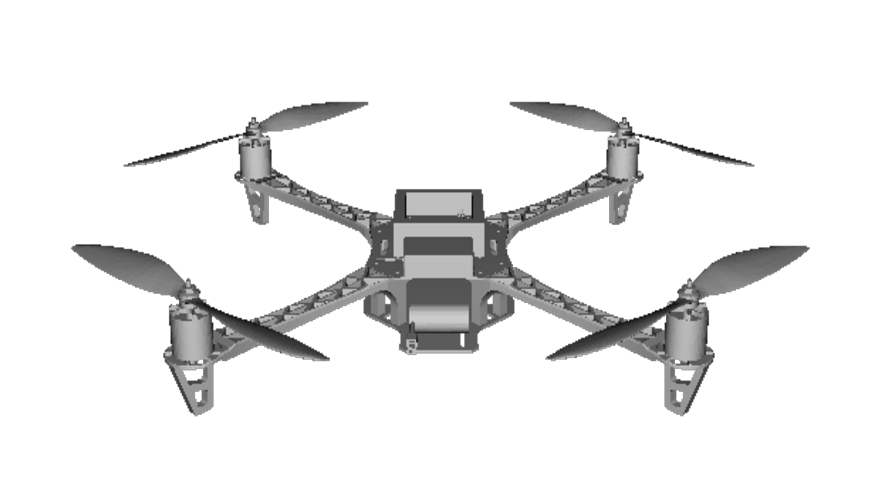
\includegraphics[width=0.6\textwidth]{uavswarm/uav}
\caption{UAV 3D model}
\label{fig:single_uav}
\end{center}
\end{figure}

\subsection{Usage}
\label{sec:uavswarm_usage}

The example is available from the INTO-CPS application menu at \emph{File>Import Example Project} or at  \url{https://github.com/into-cps/case-study\_uav\_swarm} in the \emph{master} branch. There are several subfolders for the various elements: \texttt{FMU} -- contains the various FMUs of the study; \texttt{Models} -- contains the constituent models defined using the INTO-CPS simulation technologies; \texttt{Multi-models} -- contains the multi-model definitions and co-simulation configurations -- with 3D and non-3D options; and \texttt{SysML} -- contains the SysML model defined for the study.

The \texttt{case-study\_uav\_swarm folder} can be opened in the INTO-CPS application to run various co-simulation experiments. To run a simulation, expand one of the multi-models and click `Simulate' for an experiment. 

%\subsection{INTO-CPS Technology}
%\label{sec:uavswarm_into}

\subsection{INTO-CPS SysML profile}
\label{sec:uavswarm_into_sys}

Using the INTO-SysML profile, we model a subset of the pilot study. The reason for modelling only a small subset will become clear in this section. In Figure~\ref{fig:uav_asd}, we show an Architecture Structure Diagram (ASD) depicting 3 UAVs -- each comprised of a \emph{UAVController} component and a \emph{UAV} component, a component for 3D visualisation \emph{UAV 3D}, and a \emph{UAV Global Controller} component. Each component has a large number of inputs and outputs. Briefly the \emph{UAV} has inputs for setting the pitch, yaw, roll and throttle, and outputs for the position, velocity and battery status. The \emph{UAV Controller} has the same ports, but with reversed direction and also ports to receive commands from the global controller. The optional \emph{UAV 3D} takes as input the position, pitch, yaw and roll of each UAV. Finally, the \emph{UAV Global Controller} has a collection of ports for target locations for each UAV. 

\begin{figure}[htbp]
\begin{center}
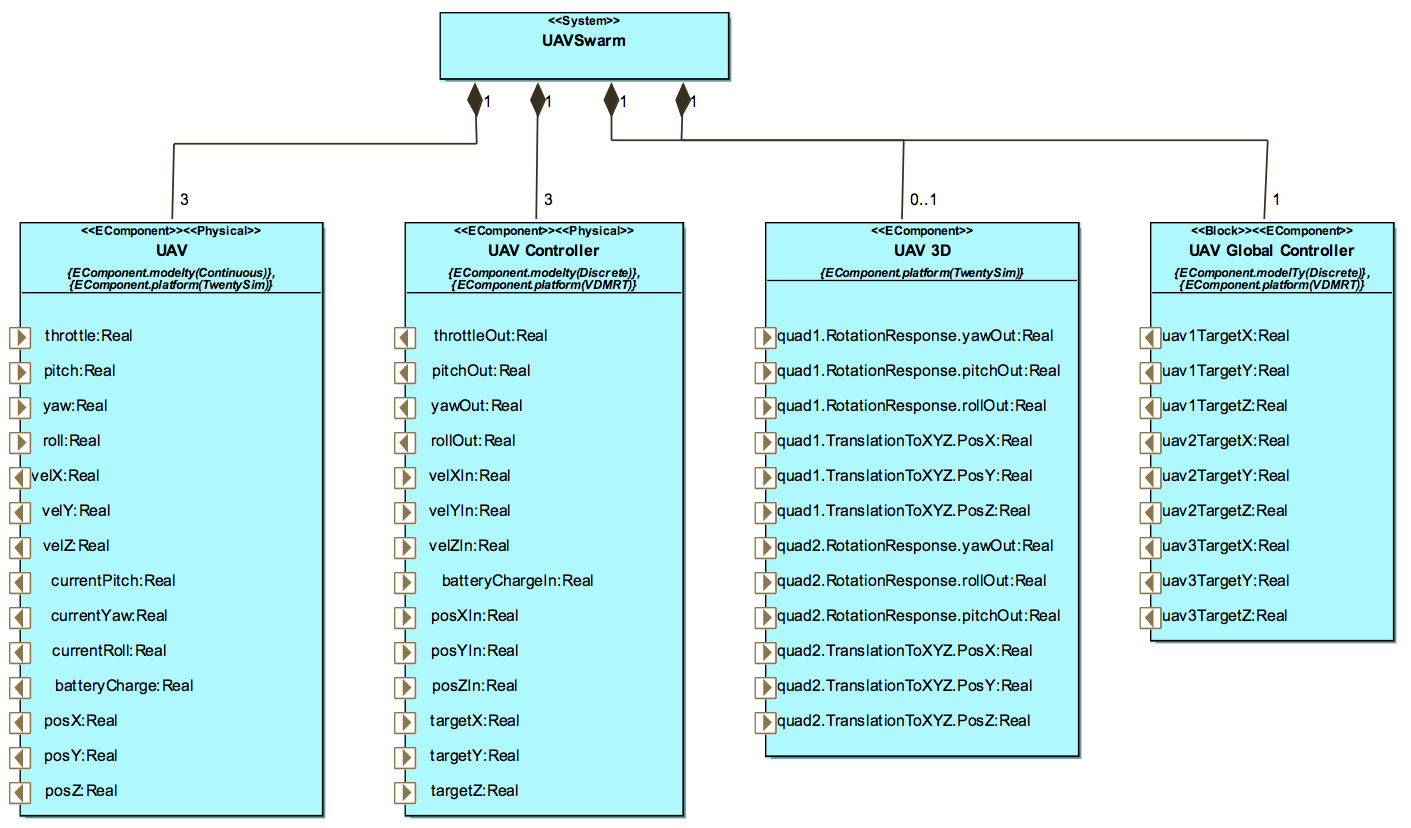
\includegraphics[width=0.95\textwidth]{uavswarm/swarm_asd}
\caption{UAV Swarm Architecture Structure Diagram}
\label{fig:uav_asd}
\end{center}
\end{figure}

Due to the large number of ports and connectors in this pilot, it is not appropriate to represent them all on the same diagram. As such, we create a single Connections Diagram (CD) per UAV each containing the same system instance (\emph{swarm : UAVSwarm}). Combining all CDs produces a complete configuration for that system instance.  The CD in Figure~\ref{fig:uav1_cd} depicts connections between the \emph{UAVController} component and a \emph{UAV} component of UAV1, and the connections to the \emph{UAV 3D} and \emph{UAV Global Controller} components related to UAV1. Note that the \emph{UAV 3D} and \emph{UAV Global Controller} instances have a subset of their ports shown.

\begin{figure}[htbp]
\begin{center}
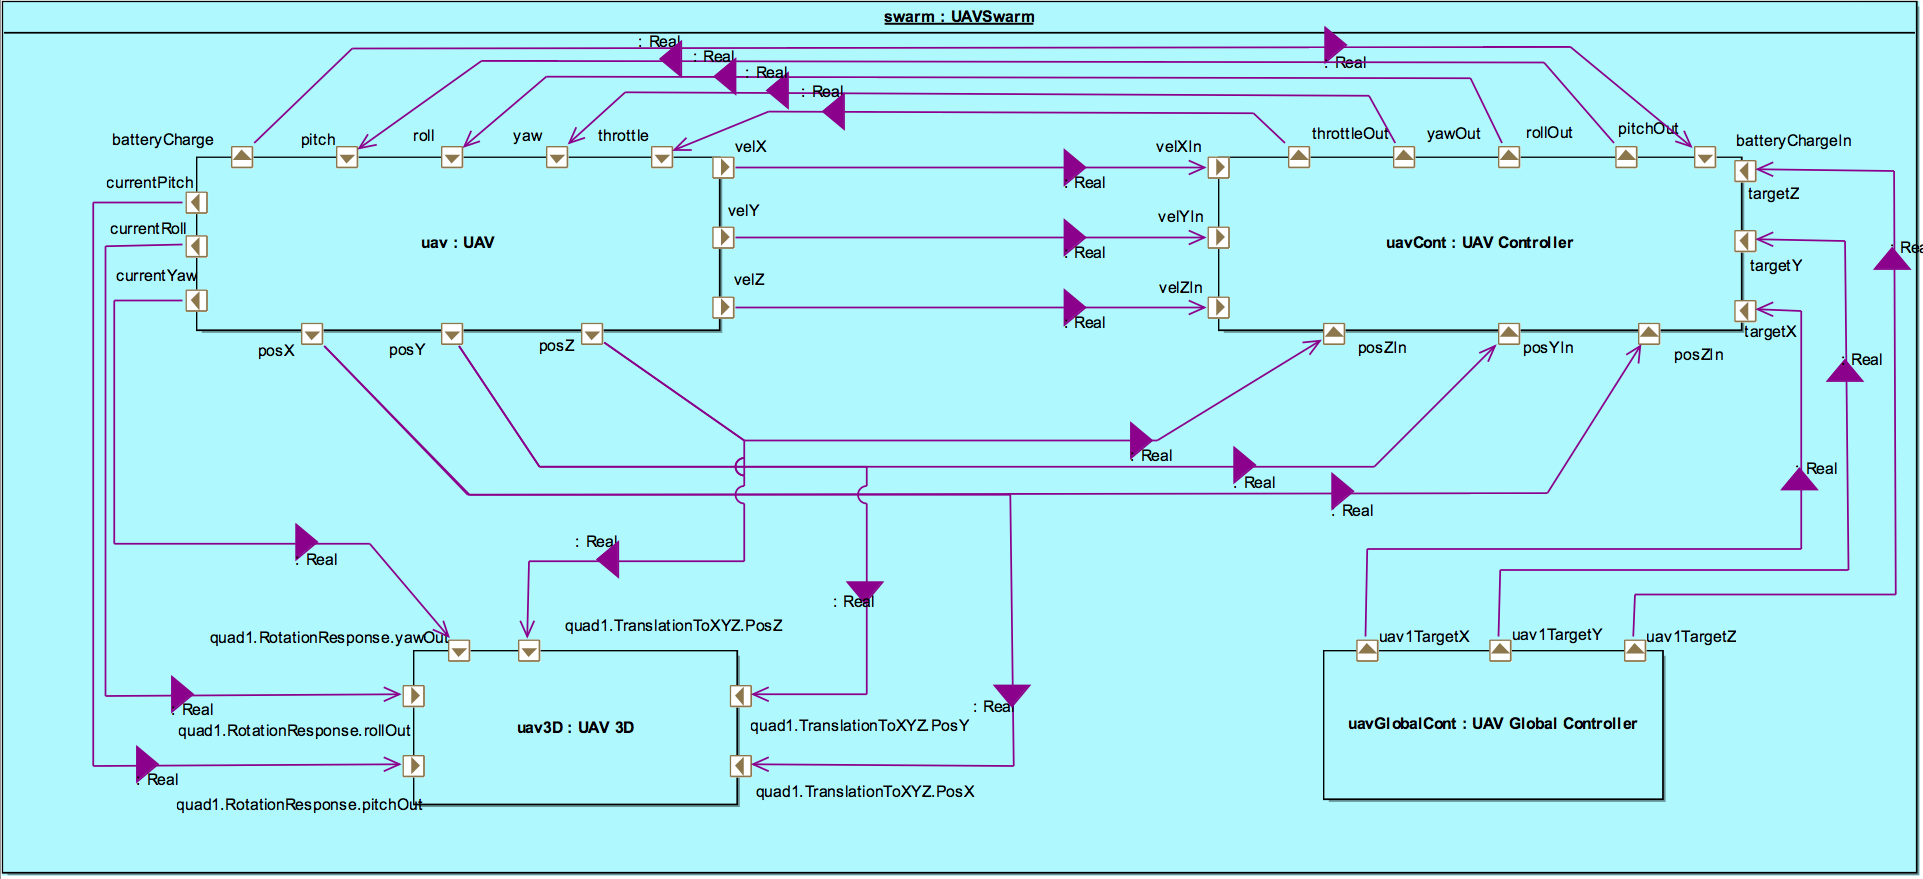
\includegraphics[width=0.95\textwidth]{uavswarm/swarm_cd}
\caption{UAV Swarm Connections Diagram showing connections relating to UAV1}
\label{fig:uav1_cd}
\end{center}
\end{figure}


\subsection{Multi-model}
\label{sec:uavswarm_into_mm}

\subsubsection{Models}
There are three models defined here (we do not include a description of the UAV 3D model.

\begin{description}
\item[UAV:] The physical model -- \emph{UAV} is defined in 20-sim. The \emph{UAV} model represents the motors, rotors, battery and implicitly the frame of the UAV. The top-level structure of the model is shown in Figure~\ref{fig:swarm-20-sim}.

\begin{figure}[htbp]
\begin{center}
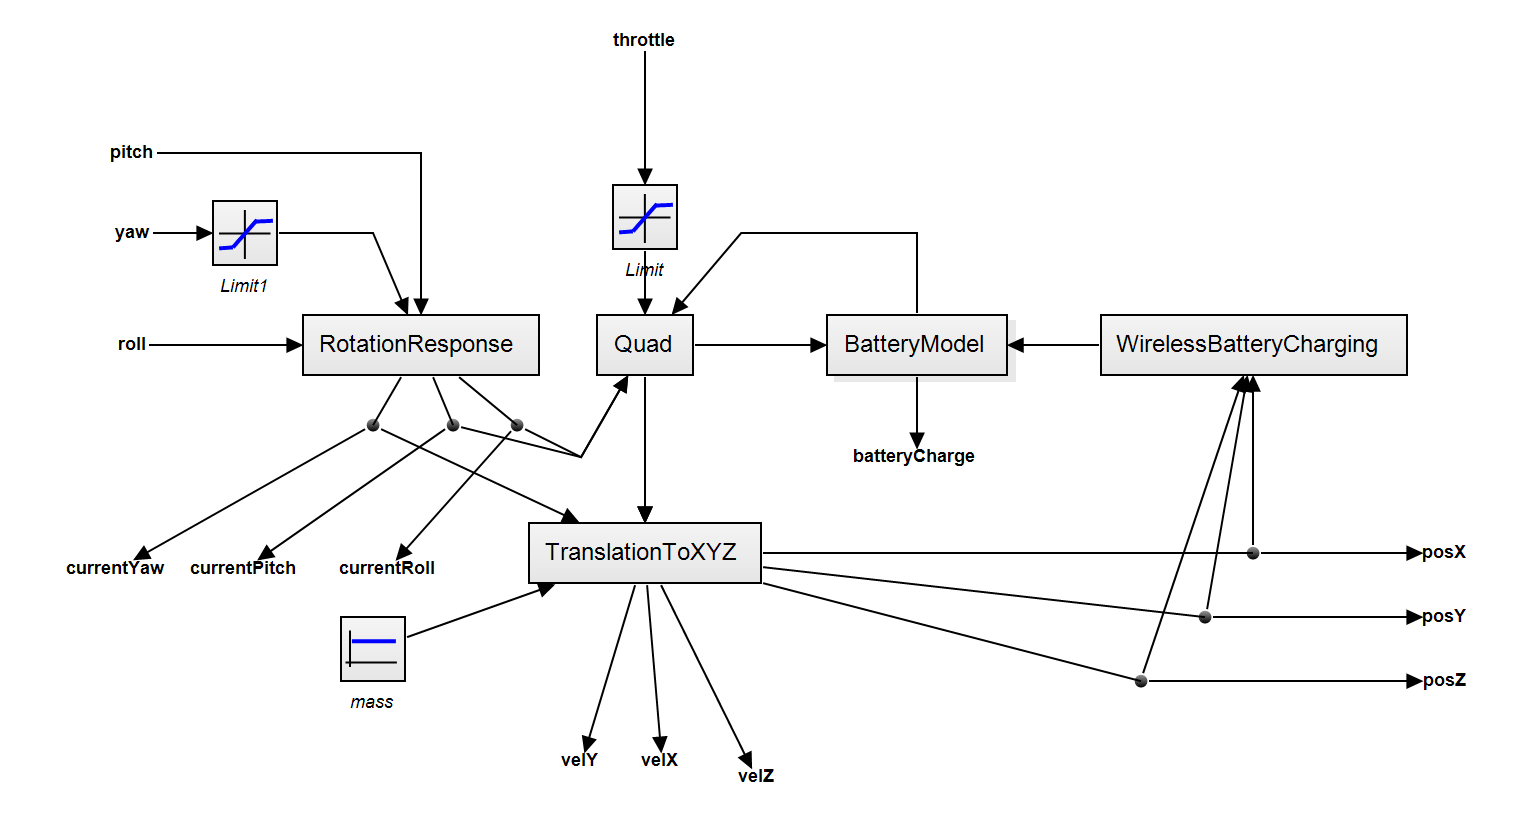
\includegraphics[width=0.9\textwidth]{uavswarm/uav-20-sim-uav}
\caption{20-sim model for UAV taking part in a Swarm}
\label{fig:swarm-20-sim}
\end{center}
\end{figure}

As can be seen from Figure~\ref{fig:swarm-20-sim}, there are several input and output signal ports -- these correspond to those ports defined in the SysML model above -- for setting the pitch, yaw and roll and reporting various aspects for control and visualisation purposes. The model is simplified and more abstract from that in Section~\ref{sec:uavsingle}, in that it is better suited to modelling shallow pitch and roll angles and contains several simplifications. The inputs from the controller enter the UAV model in two places with the pitch, roll and yaw entering the \emph{RotationResponse} block while the throttle setting enters the \emph{quad} block.  This model of the UAV abstracts away the fact of there being four distinct rotors and so a simplified model of their effects on the orientation of the UAV, so instead of torques from the four rotors being applied to the UAV body and the acceleration calculated, the \emph{RoationResponse} considers the difference between the current and requested pitch, roll and yaw rate an simulates a damped transition from the current to the requested.   The resulting orientations are sent to the \emph{quad} where they are combined with the throttle setting and battery voltage to give thrust vectors along the vertical, front and side axis of UAV.  These vectors along with the UAV yaw are sent to the \emph{translationToXYZ} where the thruse vectors are mapped onto the X,Y and Z axis and drag, accelerations, velocities and positions computed.  The final two blocks \emph{BatteryModel} and \emph{WirelessBatteryChargin} calculate the charge going into and out of the battery so that its working voltage may be output to the \emph{quad} model.

\item[UAVController:] The first of two VDM-RT models -- \emph{UAVController} -- has a similar architecture to other pilots (e.g. the line follower robot in Section~\ref{sec:linefollwerrobot}), in that the \emph{System} has an instance of a \emph{HardwareInterface} class containing ports for the inputs and outputs of the model. The \emph{System} class also has an instance of the  \emph{Controller} class, which owns several instances which sense or make changes to the environment -- they are \emph{Actuators}, \emph{Sensors} and \emph{Commands}. The controller has a collection of operations that aim to control the movement of the underlying UAV -- the top-level control loop takes the commands from the environment with target locations. Given the X, Y  and Z coordinate the UAV should meet, the controller calculates the throttle, yaw and roll to achieve the change form the current position to that target. Those values are sent on the output ports.

\begin{figure}[htbp]
\begin{center}
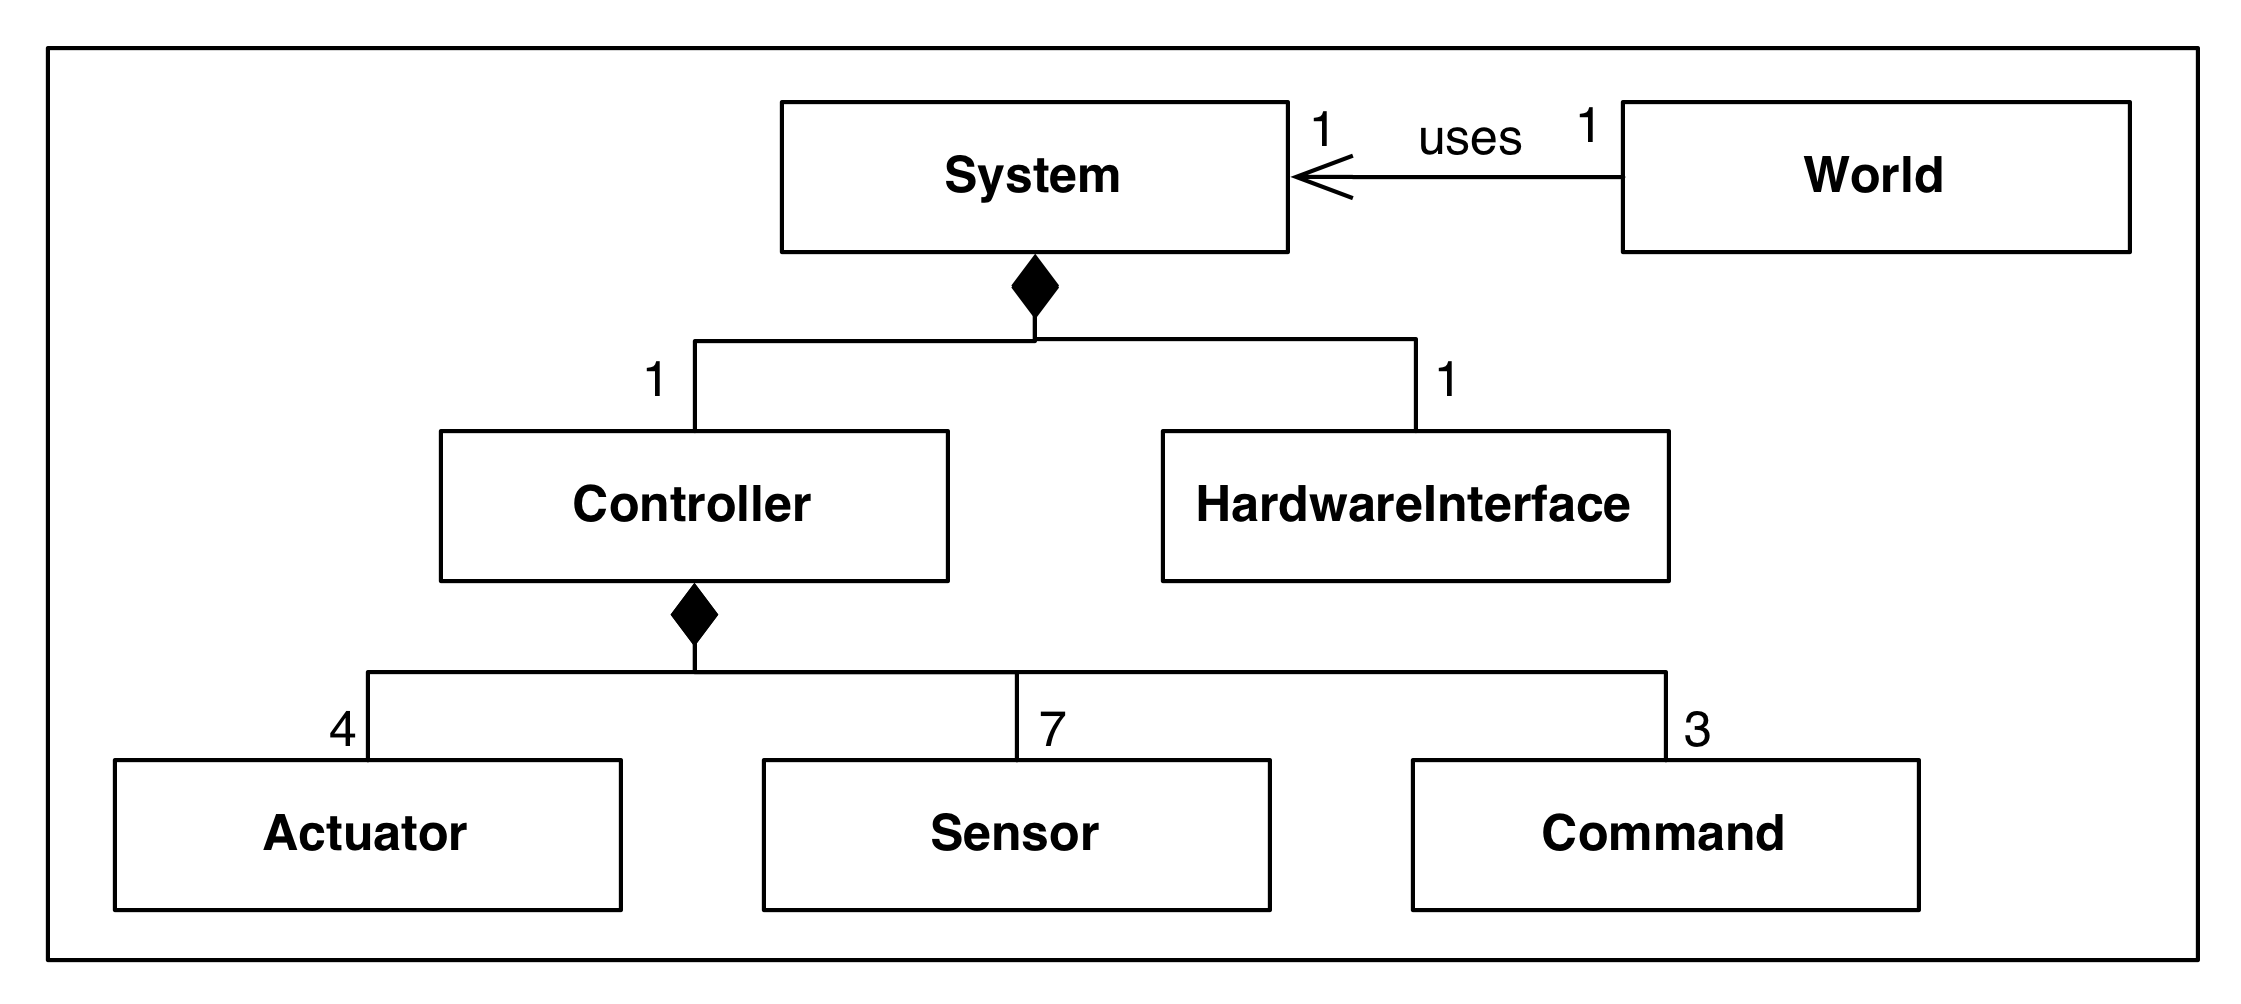
\includegraphics[width=0.8\textwidth]{uavswarm/uavcontarch}
\caption{UAV Controller architecture}
\label{fig:swarm-uav-cont}
\end{center}
\end{figure}

\item[GlobalUAVController:] The global controller for the UAV Swarm study is a simple model, which sends target locations to the different UAVs in the study at differing times. The \emph{System} class contains the \emph{HardwareInterface} class with ports for outputs of the model, and a \emph{Controller} class which owns instances of objects which set those output values. In addition, the \emph{Controller} includes a \emph{Command} class that contains the main control loop. This loop will change the target coordinates of each UAV at  different time steps, which are sent as outputs to the correct UAV.


\begin{figure}[htbp]
\begin{center}
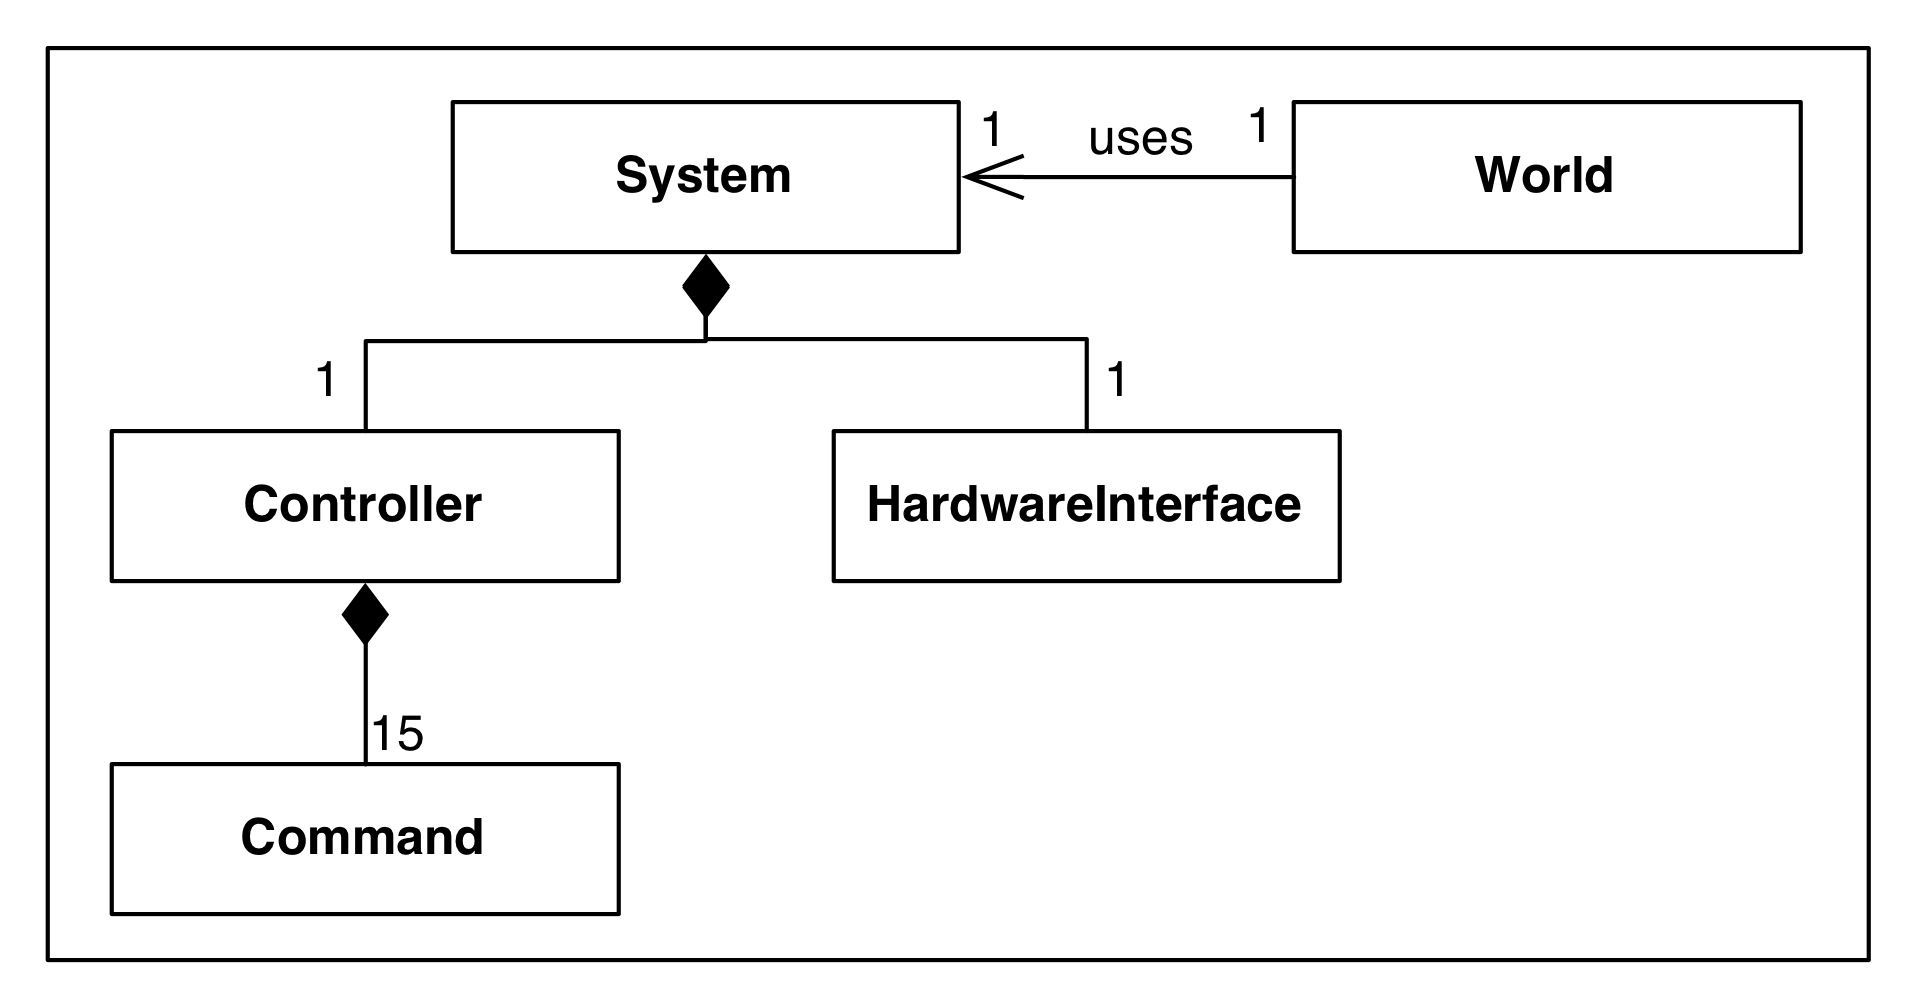
\includegraphics[width=0.7\textwidth]{uavswarm/globaluavcontarch}
\caption{Global UAV Controller architecture}
\label{fig:swarm-global-cont}
\end{center}
\end{figure}
\end{description}

\subsubsection{Configuration}

The multi-model configuration comprises a collection of connections between the FMUs. We do not use  parameters in the example. The connections may be grouped into three classes: between \emph{UAV} and \emph{UAVController}, between \emph{UAVController} and \emph{GlobalController} and \emph{UAV} to \emph{3DUAV}. These groups are repeated for each UAV in the pilot, therefore we only describe one set of connections -- see Section~\ref{sec:uavswarm_into_co} for different co-simulation experiments.

The first set is between the \emph{UAV} and \emph{UAVController}:
 \begin{itemize}
  \item from the \emph{UAV} \texttt{velX} port to the \emph{UAVController} \texttt{velXIn} port;
  \item from the \emph{UAV} \texttt{velY} port to the \emph{UAVController} \texttt{velYIn} port; 
  \item from the \emph{UAV} \texttt{velZ} port to the \emph{UAVController} \texttt{velZIn} port; 
  \item from the \emph{UAV} \texttt{batteryCharge} port to the \emph{UAVController} \texttt{batteryCharge} port;
  \item from the \emph{UAV} \texttt{posX} port to the \emph{UAVController} \texttt{posXIn} port;
  \item from the \emph{UAV} \texttt{posY} port to the \emph{UAVController} \texttt{posYIn} port; 
  \item from the \emph{UAV} \texttt{posZ} port to the \emph{UAVController} \texttt{posZIn} port; 
  \item from the \emph{UAVController} \texttt{throttleOut} port to the \emph{UAV} \texttt{throttle} port;
  \item from the \emph{UAVController} \texttt{pitchOut} port to the \emph{UAV} \texttt{pitch} port; 
  \item from the \emph{UAVController} \texttt{yawOut} port to the \emph{UAV} \texttt{yaw} port; and
  \item from the \emph{UAVController} \texttt{rollOut} port to the \emph{UAV} \texttt{roll} port.
\end{itemize}
  
The second set is between the \emph{UAVController} and \emph{GlobalController}:
\begin{itemize}
  \item from the \emph{UAVGlobalController} \texttt{uavTargetX} port to the \emph{UAVController} \texttt{targetX} port;
  \item from the \emph{UAVGlobalController} \texttt{uavTargetY} port to the \emph{UAVController} \texttt{targetY} port; and 
  \item from the \emph{UAVGlobalController} \texttt{uavTargetZ} port to the \emph{UAVController} \texttt{targetZ} port.
 \end{itemize}

The final set is between the \emph{UAV} and \emph{3DUAV}:
 \begin{itemize}
  \item from the \emph{UAV} \texttt{currentPitch} port to the \emph{3DUAV} \texttt{quad.RotationResponse.pitchOut} port;
  \item from the \emph{UAV} \texttt{currentYaw} port to the \emph{3DUAV} \texttt{quad.RotationResponse.yawOut} port;
  \item from the \emph{UAV} \texttt{currentRoll} port to the \emph{3DUAV} \texttt{quad.RotationResponse.rollOut} port;
  \item from the \emph{UAV} \texttt{posX} port to the \emph{3DUAV} \texttt{quad.TranslationToXYZ.PosX} port;
  \item from the \emph{UAV} \texttt{posY} port to the \emph{3DUAV} \texttt{quad.TranslationToXYZ.PosY} port; and 
  \item from the \emph{UAV} \texttt{posZ} port to the \emph{3DUAV} \texttt{quad.TranslationToXYZ.PosZ} port.
\end{itemize}


\subsection{Co-simulation}
\label{sec:uavswarm_into_co}

Four multi-model configuration variations are defined to enable different co-simulation experiments. Those different multi-models vary by the number of UAVs (the number of \emph{UAV} and \emph{UAVController} FMU instances) and the inclusion of the \emph{3DUAV} FMU for visualisation:

\begin{description}
  \item[3-UAV-3D] This multi-model comprises 4 FMUs: 3 instances of \emph{UAV.fmu}; 3 of \emph{UAVController.fmu}; 1 instance of \emph{3DanimationFMU.fmu}; and 1 instance of \emph{UAVGlobalController.fmu}. The multi-model has a co-simulation experiment with a run time of 10 seconds and with a variable step size. The 3D visualisation shows the flight paths of the UAVs.
  \item[3-UAV-Non-3D] The 3-UAV non-3D multi-model is the same as the above study, however without the  \emph{3DanimationFMU.fmu} instance. Without the 3D view, livestream values are enabled for the x-position of the 3 UAVs -- this may be changed.
  \item[5-UAV-3D] The 5-UAV-3D multi-model is the same as in the 5-UAV-3D version, however with 5 instances of \emph{UAV.fmu} and \emph{UAVController.fmu}. 
  \item[5-UAV-Non-3D] Again,  the 5-UAV-Non-3D multi-model is the same as in the 5-UAV-Non-3D version, however with 5 instances of \emph{UAV.fmu} and \emph{UAVController.fmu}. 
\end{description}

The 3D visualisation offered by those 3D multi-models opens a 3D visualisation window as shown in Figure~\ref{fig:swarm-uav-vis} which depicts the state of the swarm as the simulation progresses. It should be noted that the FMU has a fixed number of UAV objects, therefore the FMU must be extended to handle a greater number of UAVs in a swarm.

\begin{figure}[htbp]
\begin{center}
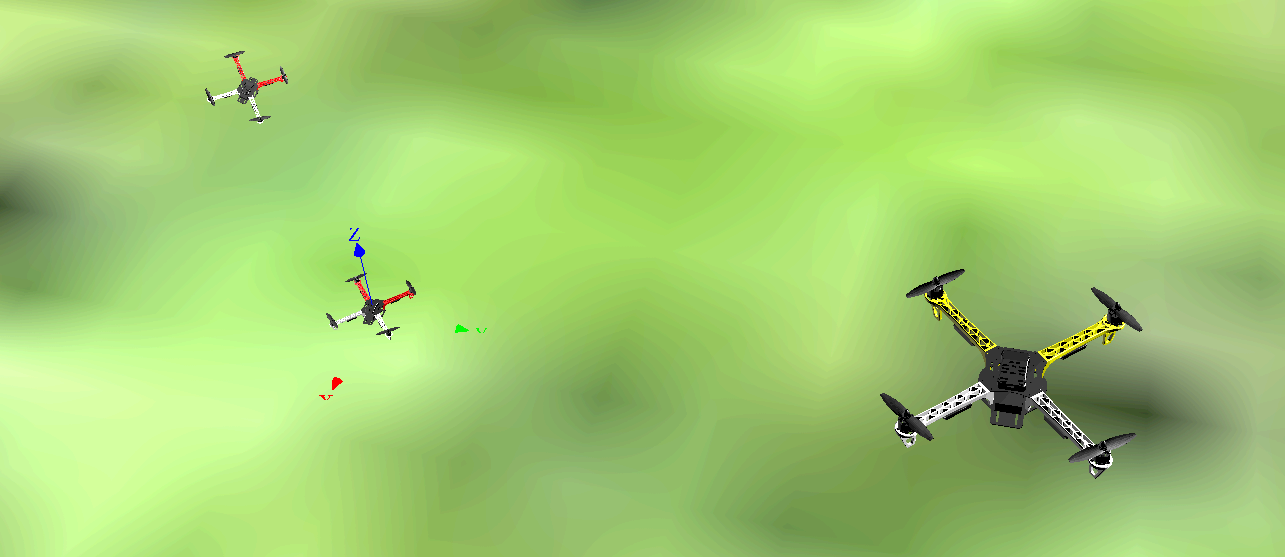
\includegraphics[width=0.8\textwidth]{uavswarm/uav-3d1}
\caption{UAV Swarm visualisation}
\label{fig:swarm-uav-vis}
\end{center}
\end{figure}

\subsection{Analyses and Experiments}
\label{sec:uavswarm_into_analysis}


\subsubsection{Test Automation and Model Checking}
\label{sec:uavswarm_ta}

\graphicspath{ {./uavswarm/TA/} }
Unlike multi-model that has three or five UAVs in a swarm, we use two UAVs in the test model. This is because multiple instances are not supported in the test model. For each instance, we have to create a new block and have all similar local variables and state machine diagrams in this block. More instances will complicate the test model as well as solving of test cases in the SMT solver. Eventually, we choose two UAVs to keep the test model relatively simple and still more than one UAV.

In addition, communication between controllers through the Ether is also introduced.  Therefore, the system covered in our test model is composed of
\begin{itemize}
    \item two physical \emph{UAVs},
    \item two discrete \emph{UAV Controllers} (one controller for each UAV),
    \item a discrete \emph{UAV Global Controller},
    \item a \emph{Ether} model through which
        \begin{itemize}
            \item \emph{Global Controller} is able to send target positions to \emph{UAV Controllers} by unicast, and
            \item \emph{UAV Controllers} are able to broadcast their current positions to other \emph{UAV Controllers} and \emph{Global Controller}.
        \end{itemize}
\end{itemize}

\paragraph{Test Model}
Our test model aims to model the discrete part of the UAV swarm study. To be more specific, it includes two \emph{UAV Controllers}, a \emph{Global Controller} and a \emph{Ether} which is described in Section~\ref{sec:ether}. The physical \emph{UAVs} are regarded as the test environment of the model.

\subparagraph{Inputs and Outputs}
The \emph{SystemUnderTest} receives the following inputs (stimuli) from the \emph{TestEnvironment}:
\begin{itemize}
    \item $targetX1$, $targetY1$, and $targetZ1$: target positions on X, Y and Z respectively for the first \emph{UAV} (\emph{UAV1}), 
    \item $targetX2$, $targetY2$, and $targetZ2$: target positions on X, Y and Z respectively for the second \emph{UAV} (\emph{UAV2}).
%\end{itemize}
%
%The \emph{SystemUnderTest} receives the following inputs (stimuli) from the \emph{TestEnvironment} (\emph{UAVs}):
%\begin{itemize}
    \item $velX1$, $velY1$, and $velZ1$: current velocity of \emph{UAV1} on the X, Y and Z axes respectively,
    \item $posX1$, $posY1$, and $posZ1$: current position of \emph{UAV1} on the X, Y and Z axes respectively, 
    \item $batteryCharge$: battery status of \emph{UAV1},
    \item $velX2$, $velY2$, and $velZ2$: current velocity of \emph{UAV2} on the X, Y and Z axes respectively,
    \item $posX2$, $posY2$, and $posZ2$: current position of \emph{UAV2} on the X, Y and Z axes respectively,
    \item $batteryCharge$: battery status of \emph{UAV2}.
\end{itemize}

The \emph{SystemUnderTest} provides the following observable outputs to the \emph{TestEnvironment}:
\begin{itemize}
    \item $pitchOut1$ and $pitchOut2$: pitch set point for \emph{UAV1} and \emph{UAV2} respectively,
    \item $throttleOut1$ and $throttleOut2$: throttle set point for \emph{UAV1} and \emph{UAV2} respectively,
    \item $rollOut1$ and $rollOut2$: roll set point for \emph{UAV1} and \emph{UAV2} respectively.
\end{itemize}

\subparagraph{Interfaces}
In addition to the interfaces between \emph{SystemUnderTest} and \emph{TestEnvironment} for inputs and outputs, six extra interfaces, shown in Figure~\ref{fig:uav_swarm_sut_intfs}, are defined for connections between all controllers and \emph{Ether}.
\begin{itemize}
    \item \emph{GlobalEtherInIF} and \emph{GlobalEtherOutIF}: interfaces for connections between \emph{Global Controller} and \emph{Ether}. In the name of the interfaces, \emph{in} and \emph{out} mean inputs to and outputs from \emph{Ether}. Therefore, \emph{GlobalEtherInIF} is an interface from \emph{Global Controller} to \emph{Ether}, and \emph{GlobalEtherOutIF} is an interface from \emph{Ether} to \emph{Global Controller}. For the variable names in the interfaces, \emph{a} denotes the address part and \emph{p} denotes the payload part. $GEin1a$, $GEin1p1$, $GEin1p2$ and $GEin1p3$ in \emph{GlobalEtherInIF} compose a package in which there are one integer for the address and three doubles for the payload. But \emph{GlobalEtherOutIF} contains two packages, which means \emph{Ether} can send two packages to \emph{Global Controller} once but it can only receive one package from \emph{Global Controller}.
    \item \emph{UAV1EtherInIF} and \emph{UAV1EtherOutIF}: interfaces for connections between \emph{UAV1 Controller} and \emph{Ether}. 
    \item \emph{UAV2EtherInIF} and \emph{UAV2EtherOutIF}: interfaces for connections between \emph{UAV2 Controller} and \emph{Ether}. 
\end{itemize}

\begin{figure}[htb!]
    \centering
	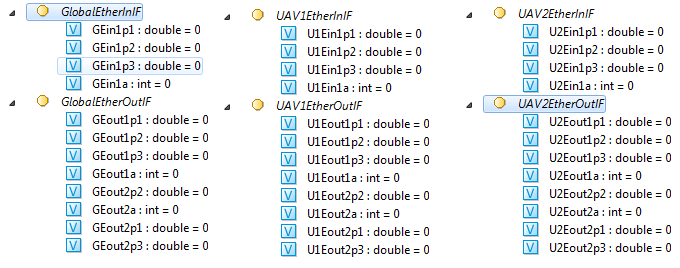
\includegraphics[width=1.0\textwidth]{uav_swarm_sut_intfs}
    \caption{Interfaces in \emph{SystemUnderTest}}
    \label{fig:uav_swarm_sut_intfs}
\end{figure}

\subparagraph{\emph{SystemUnderTest}}
\emph{SystemUnderTest} is composed of two \emph{UAV Controllers}, a \emph{Global Controller} and a \emph{Ether}. The architecture structure diagram of \emph{SystemUnderTest} is shown in Figure~\ref{fig:uav_swarm_sut_sad} and the connection diagram is illustrated in Figure~\ref{fig:uav_swarm_sut_cd}. From the connection diagram, we can see that all controllers are connected to \emph{Ether} directly and each of them has two connections to \emph{Ether} in two directions. Therefore they are able to communicate each other in two directions via \emph{Ether}. 

\begin{figure}[htb!]
    \centering
	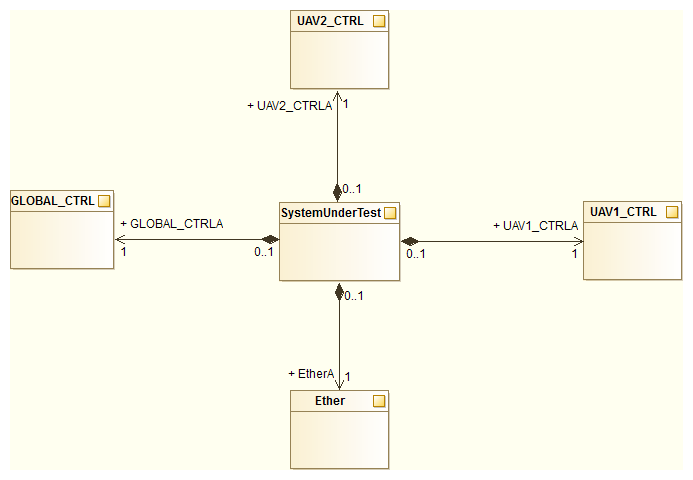
\includegraphics[width=1.0\textwidth]{uav_swarm_sut_sad}
    \caption{Architecture Structure Diagram of \emph{SystemUnderTest}}
    \label{fig:uav_swarm_sut_sad}
\end{figure}

\begin{figure}[htb!]
    \centering
	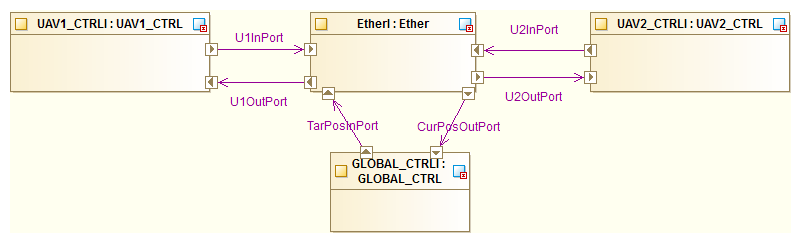
\includegraphics[width=1.0\textwidth]{uav_swarm_sut_cd}
    \caption{Connection Diagram of \emph{SystemUnderTest}}
    \label{fig:uav_swarm_sut_cd}
\end{figure}

\subparagraph{Ether}
In order to contain messages for communication into the payload part of packages, the package structure is revised based on that given in Section~\ref{sssec:ether_encoding}.

A package is composed of two parts: address and payload. The address part is encoded in one integer and the payload part is in three doubles.
\begin{itemize}
    \item Address (32-bit int): high 24 bits are always 0, low 8 bits are split into two 4-bit parts (one for the destination port and one for the source port). 
        \begin{itemize}
            \item 0xF: for broadcast;
            \item 0x1-0xE: port 1 - port 15;
            \item 0x0: no message signal (used for the polling method to identify a valid package);
            \item In this case, 0x1 and 0x2 are used to identify \emph{UAV1 Controller} and \emph{UAV2 Controller}, 0xE for \emph{Global Controller}, and 0xF for broadcast.
        \end{itemize}
    \item Payload (three doubles): for the position or velocity on X, Y, and Z axes.
\end{itemize}

The state machine diagram of Ether is illustrated in Figure~\ref{fig:uav_swarm_sut_ether_sm}. After the \T{Init} state, it enters the \T{IDLE} state with the timer variable $t$ reset. Then if 10 ms is elapsed, the transition to \T{PreUpdate} fires. It checks all input packages from \emph{Global Controller} and \emph{UAV Controllers}, then copies them into output packages of the expected ports. In the end, the state machine returns to \T{IDLE} and waits for the next loop.
\begin{figure}[htb!]
    \centering
	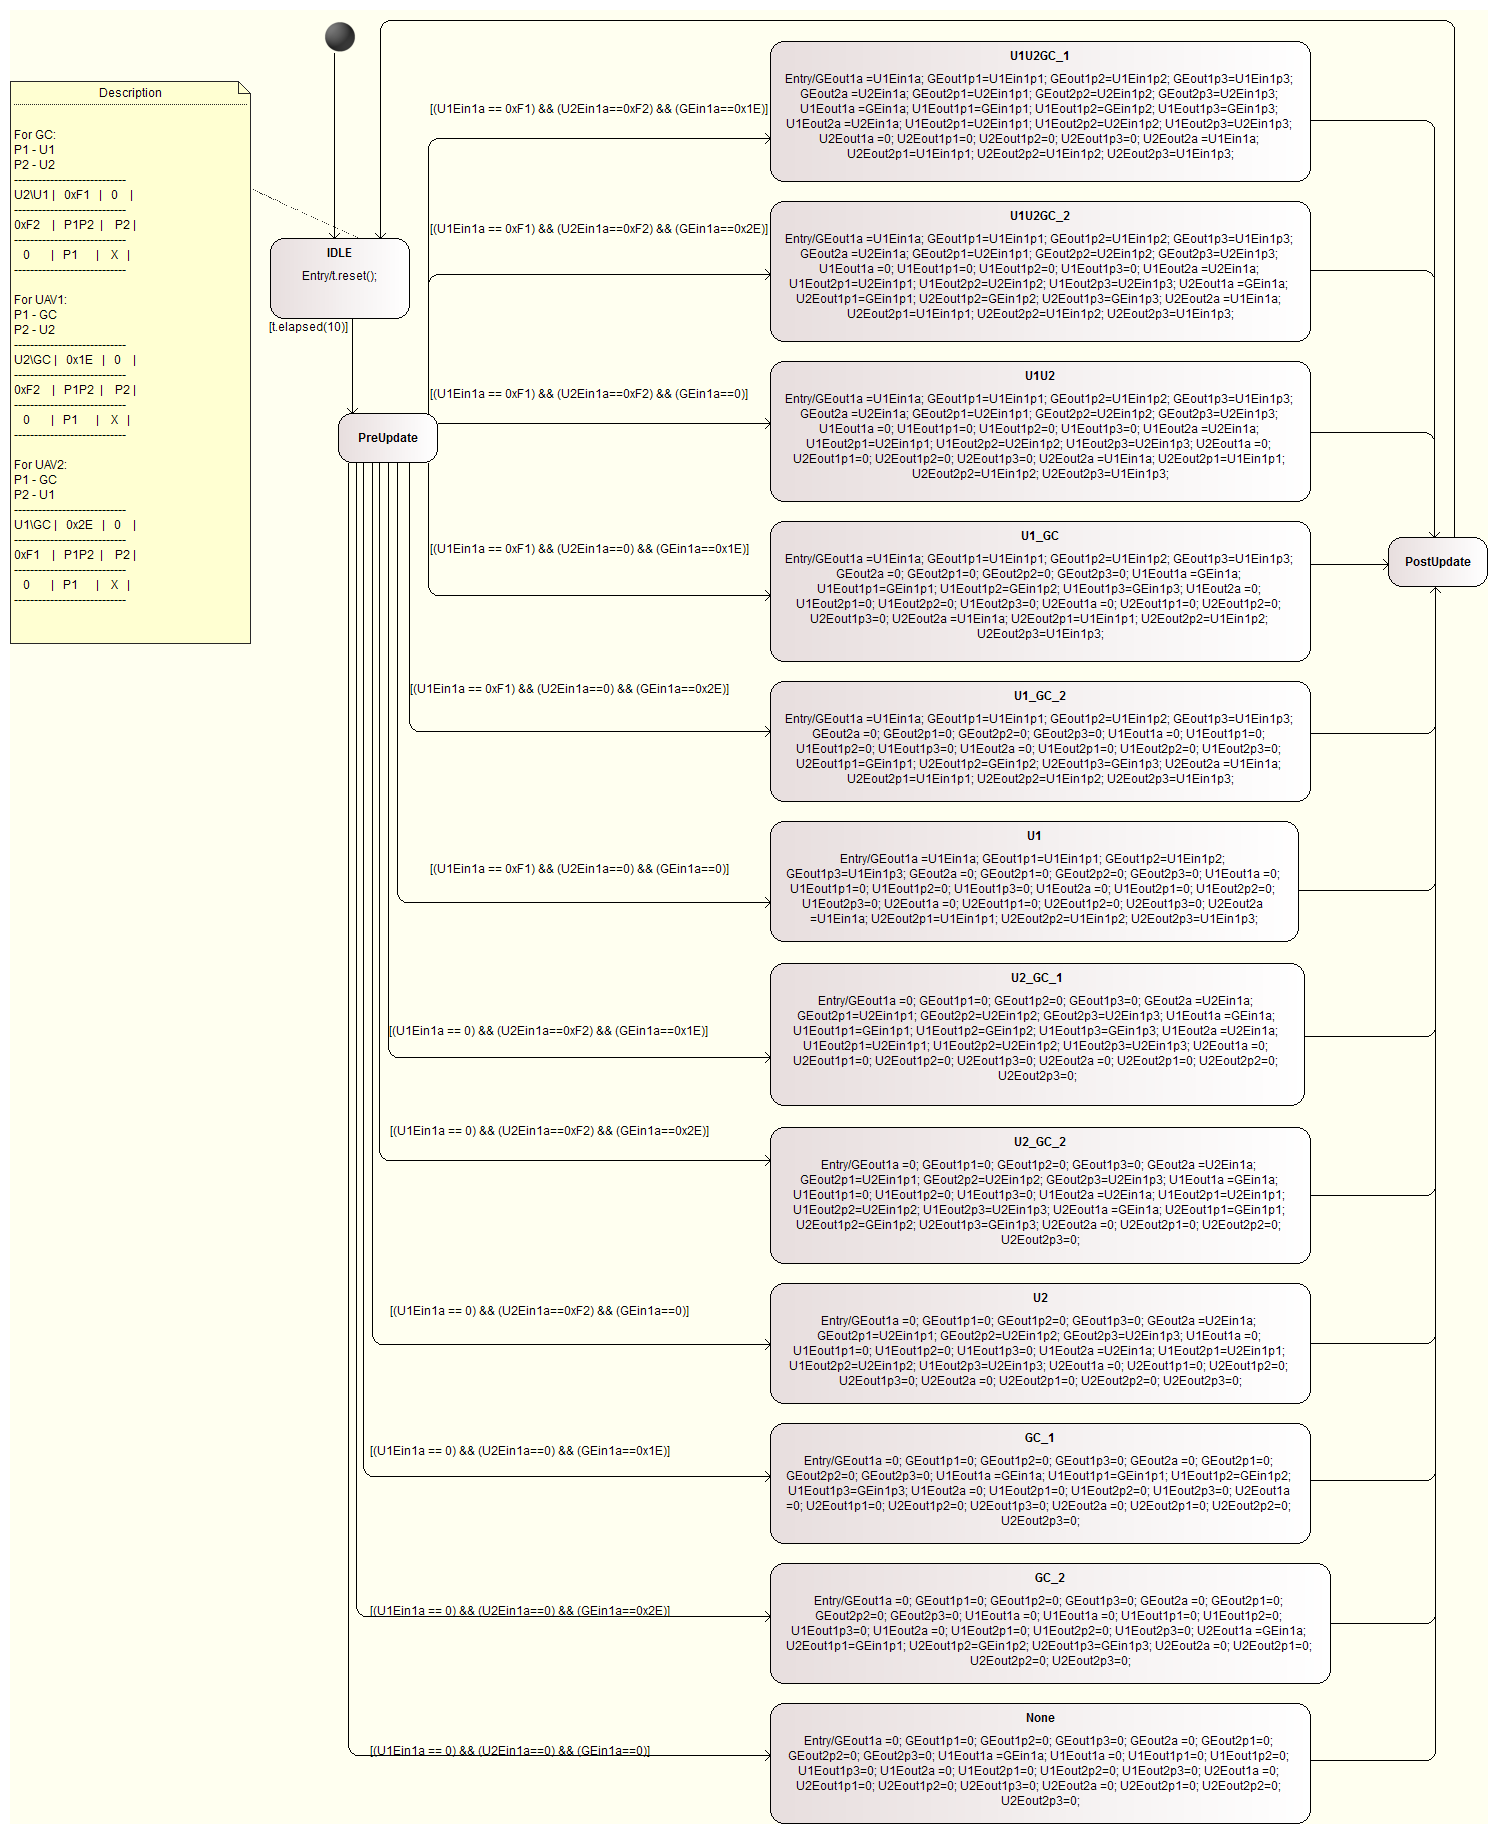
\includegraphics[width=1.0\textwidth]{uav_swarm_sut_ether_sm}
    \caption{State Machine Diagram of Ether}
    \label{fig:uav_swarm_sut_ether_sm}
\end{figure}

\subparagraph{\emph{UAV1 Controller}}
{Constant variables and local variables} of \emph{UAV1} are shown in Figure~\ref{fig:uav_swarm_uavctrl_var}.

\begin{figure}[htb!]
    \centering
	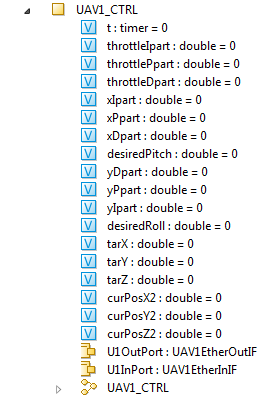
\includegraphics[width=0.4\textwidth]{uav_swarm_sut_uavctrl_var}
    \caption{Variables of UAV Controller}
    \label{fig:uav_swarm_uavctrl_var}
\end{figure}

It is worth noting that three local variables ($curPosX2$, $curPosY2$, and $curPosZ2$) are used to store current positions of \emph{UAV2}. In other words, \emph{UAV1} is aware of the position of \emph{UAV2}. These variables are updated from the packages broadcast from \emph{UAV2} through \emph{Ether}.

The state machine diagram is illustrated in Figure~\ref{fig:uav_swarm_uavctrl_sm}. Most of the time, the state machine resides in the \T{Waiting} state. And every 40 ms it starts to process.
\begin{itemize}
    \item Firstly, it is going to update its own target position from the \emph{Global Controller} and current positions of \emph{UAVs} according to incoming packages from \emph{Ether}. That is specified in the states between \T{PreUpdateTargetPos} and \T{PostUpdateTarCurPos},
    \item Then, it broadcasts its own current position in the \T{PostUpdateTarCurPos} state through \emph{Ether},
    \item Afterwards, it starts to update the parameters of the \emph{PID} controller. The entry of the state \T{PreThrottle} calculates the $throttleIpart$ and $throttlePpart$ while the transition from it to the state \T{PostThrottle} updates $throttleDpart$. Finally, the entry of \T{PostThrottle} sets the output variable $throttleOut$. The states \T{PrePitch} and \T{PostPitch}, and the states \T{PreRoll} and \T{PostRoll} are similar.
    \item Eventually, the state machine returns back to the \T{Waiting} state and waits for the next loop.
\end{itemize}


\begin{figure}[htb!]
    \centering
    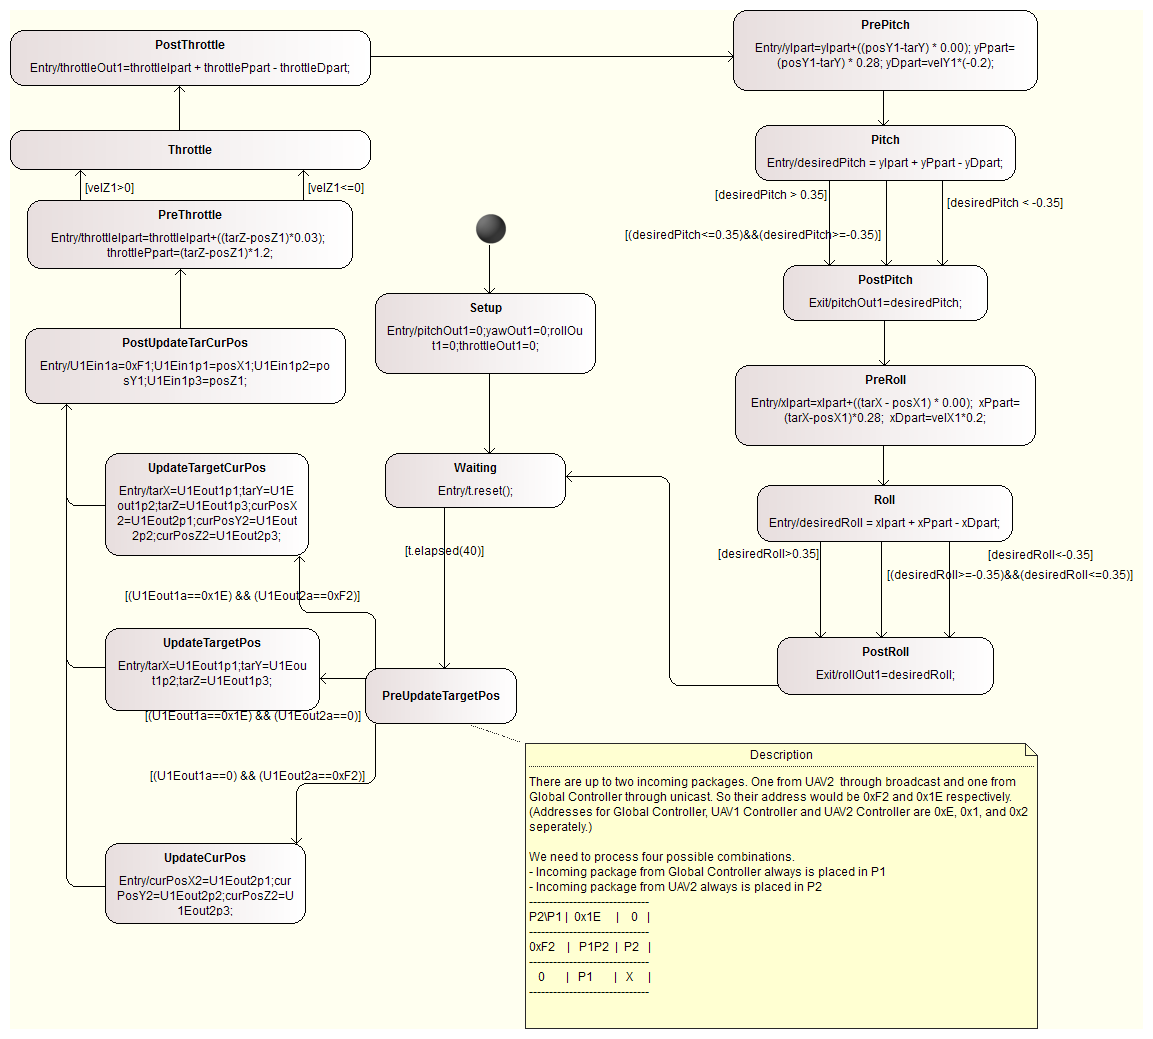
\includegraphics[width=1.0\textwidth]{uav_swarm_sut_uavctrl_sm}
    \caption{State Machine Diagram of UAV\_CTRL}
    \label{fig:uav_swarm_uavctrl_sm}
\end{figure}

\subparagraph{\emph{UAV2 Controller}}
The \emph{UAV2 Controller} model is very similar to that of the \emph{UAV1 Controller}.

\subparagraph{\emph{Global Controller}}
The \emph{Global Controller} model has six local variables (($curPosX1$, $curPosY1$, $curPosZ1$, $curPosX2$, $curPosY2$, and $curPosZ2$) to keep current positions of \emph{UAV1} and \emph{UAV2}. They are updated from broadcast packages of \emph{UAV1} and \emph{UAV2}.

The \emph{Global Controller} intends to send target positions to both \emph{UAV1} and \emph{UAV2} in each loop (40 ms). Then from the \emph{UAV Controllers} aspect, they get their target position almost at the same time because they start to process inputs every 40 ms as well. Furthermore, since one controller is able to send only one package each time to \emph{Ether} and the processing interval of \emph{Ether} is 10 ms, we need to send target positions to \emph{UAV1} and \emph{UAV2} separately with an interval of more than 10 ms. In the end, we use timing shown in the state machine diagram of \emph{Global Controller} in Figure~\ref{fig:uav_swarm_globalctrl_sm}. Its state machine loops every 40 ms too. \emph{Global Controller} sends the target position to \emph{UAV1} at 15 ms, the target position to \emph{UAV2} at 30 ms, and check incoming packages from \emph{Ether} at 40 ms.
\begin{figure}[htb!]
    \centering
	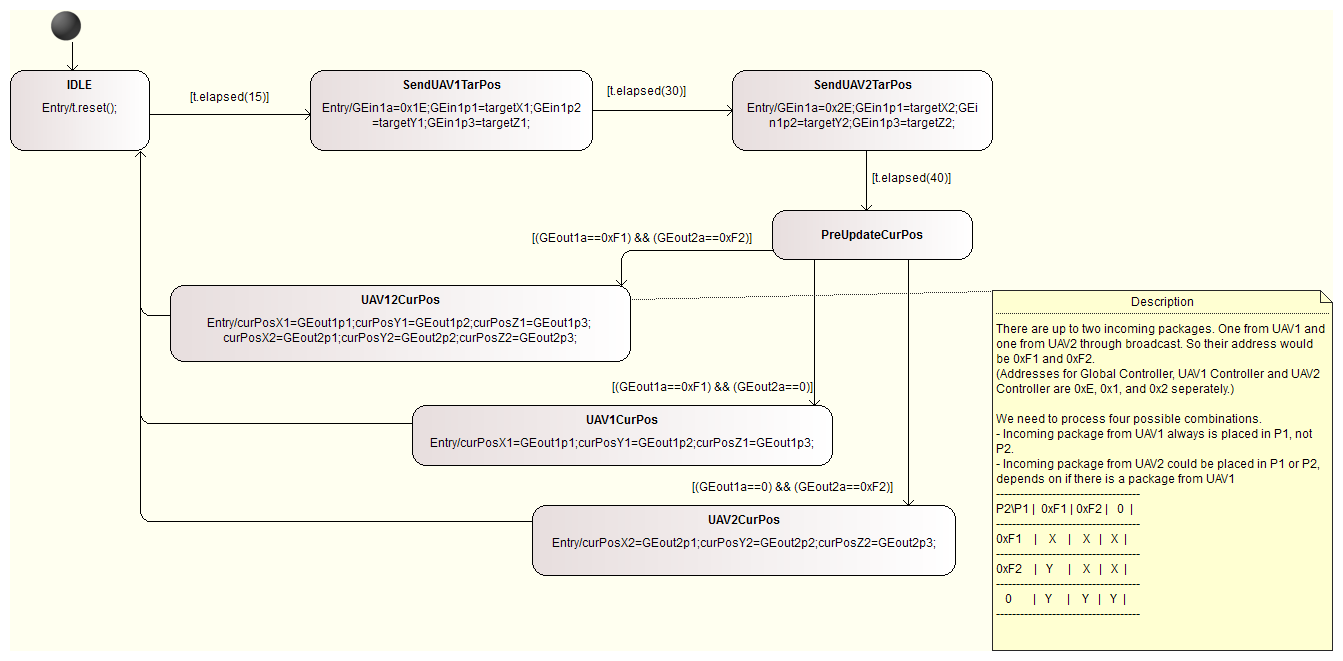
\includegraphics[width=1.0\textwidth]{uav_swarm_sut_globalctrl_sm}
    \caption{State Machine Diagram of GLOBAL\_CTRL}
    \label{fig:uav_swarm_globalctrl_sm}
\end{figure}

\subparagraph{\emph{TestEnvironment}}
We use a state machine diagram of a block \emph{TESim} in \emph{TestEnvironment} to simulate input sequences of target positions to \emph{SystemUnderTest}, which is showed in Figure~\ref{fig:uav_swarm_te_tesim_sm}.
\begin{figure}[htb!]
    \centering
	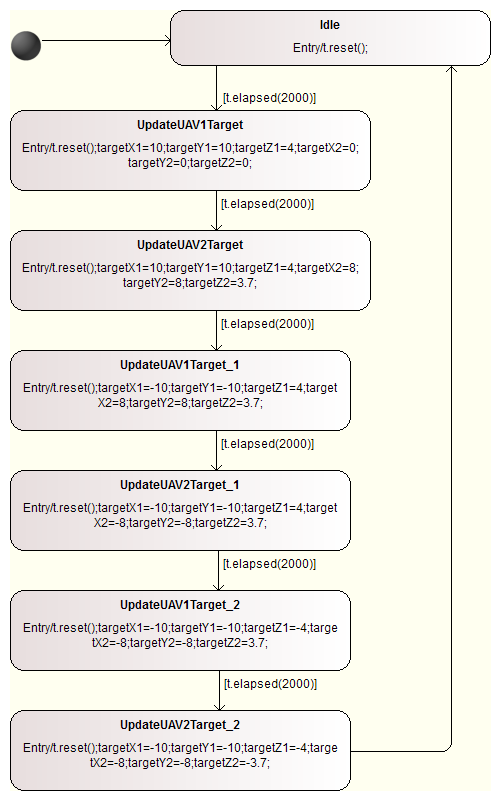
\includegraphics[width=0.7\textwidth]{uav_swarm_te_tesim_sm}
    \caption{State Machine Diagram of \emph{TESim}}
    \label{fig:uav_swarm_te_tesim_sm}
\end{figure}

The target positions of \emph{UAV1} and \emph{UAV2} specified in the state machine diagram are illustrated in Figure~\ref{fig:uav_swarm_te_tesim_target1} and Figure~\ref{fig:uav_swarm_te_tesim_target2}.
\begin{figure}[htb!]
    \centering
	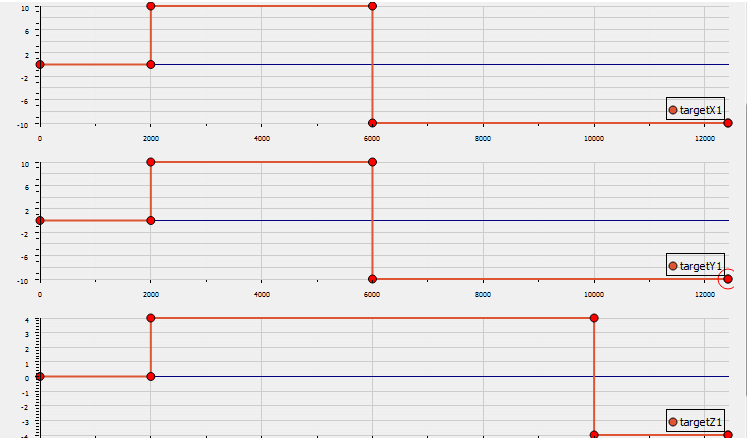
\includegraphics[width=1.0\textwidth]{uav_swarm_te_tesim_target1}
    \caption{Simulated Target Positions for \emph{UAV1}}
    \label{fig:uav_swarm_te_tesim_target1}
\end{figure}

\begin{figure}[htb!]
    \centering
	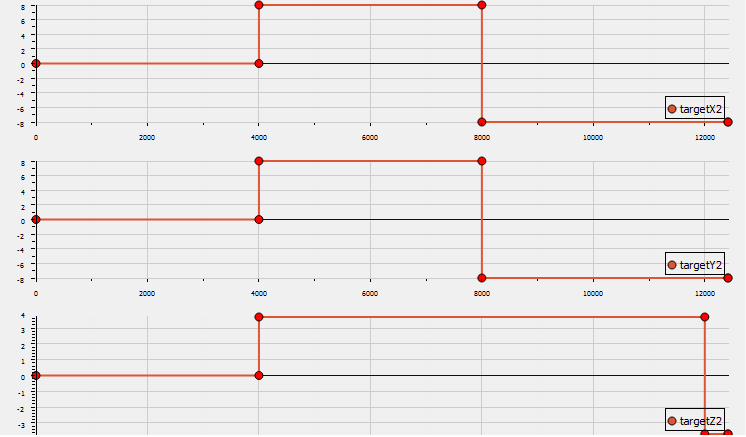
\includegraphics[width=0.9\textwidth]{uav_swarm_te_tesim_target2}
    \caption{Simulated Target Positions of \emph{UAV2}}
    \label{fig:uav_swarm_te_tesim_target2}
\end{figure}

\paragraph{Model Checking}
We set ``BMC steps'' to 50. The properties below are checked to hold in 50 steps.

\begin{description}
    \item[P0] Livelock property by the \B{Check Mode} function on RT-Tester.
\begin{verbatim}
Check static model semantics ...done.
- IMR.SystemUnderTest.EtherI... [PASS]
- IMR.SystemUnderTest.GLOBAL_CTRLI... 
[LIVELOCK_CHECK] Could not get value for the lower bound 
of the symbol IMR.SystemUnderTest.GLOBAL_CTRLI.curPosX2.
\end{verbatim}
\begin{itemize}
    \item because in the test model, these variables are given a ``RESTRICTED'' stereotype but minimum and maximum values are not specified,
    \item after removing this stereotype for each variable (except input and output variables), it is fixed and the check is passed.
\end{itemize}
\begin{verbatim}
Check static model semantics ...done.
- IMR.SystemUnderTest.EtherI...  [PASS]
- IMR.SystemUnderTest.GLOBAL_CTRLI... [PASS]
- IMR.SystemUnderTest.UAV1_CTRLI... [PASS]
- IMR.SystemUnderTest.UAV2_CTRLI... [PASS]
- IMR.TestEnvironment.tesim... [PASS]
\end{verbatim}

    \item[P1] \emph{Global Controller} sends packages only to \emph{UAV1 Controller} or \emph{UAV2 Controller}.
\begin{verbatim}
Globally ([IMR.out11a != 33] && [IMR.out11a != 34] && 
    [IMR.out21a != 17] && [IMR.out21a != 18])
\end{verbatim}

    \item[P2] All controllers could be in \T{Idle} at the same time.
\begin{verbatim}
Finally ([IMR.SystemUnderTest.End1I.End.Idle
    && IMR.SystemUnderTest.EtherI.Ether.Idle
    && IMR.SystemUnderTest.End2I.End.Idle])
\end{verbatim}

    \item[P3] A broadcast package would never be received by its source port.
\begin{verbatim}
Globally ([IMR.out11a != 241] && [IMR.out21a != 242])
\end{verbatim}
\end{description}

\paragraph{A Manual Implementation of SUT}
This SUT is composed of four modules (\emph{Global Controller}, \emph{Ether}, \emph{UAV1 Controller}, and \emph{UAV2 Controller}). And each of them corresponds to one controller in the test model and is wrapped in its own FMU in testing. 

%%\subparagraph{A Combined SUT with one FMU}
%%This SUT only has one FMU which implements the \emph{Global Controller} and two \emph{UAV Controllers} together without \emph{Ether}. Communication between \emph{Global Controller} and \emph{UAV Controllers} are merely through shared variables because all controllers are implemented in a same program.
%The source code is listed as follows.
%
%\lstset{language=C,
%    basicstyle=\footnotesize\ttfamily,
%    keywordstyle=\color{blue}\ttfamily,
%    stringstyle=\color{red}\ttfamily,
%    commentstyle=\color{green}\ttfamily,
%    morecomment=[l][\color{magenta}]{\#},
%    tabsize=2
%}
%
%\begin{lstlisting}
%
%#include <stdio.h>
%#include <sys/time.h>
%#include <sys/types.h>
%#include "uav_swarm_ctrl.h"
%
%#define _ms( t ) ( (t) * 1000 )
%
%VSTimer_t t;
%
%void reset( VSTimer_t* timer)
%{
%	struct timeval now;
%	ti_gettimeofday( &now, NULL );
%	*timer = now.tv_sec * 1000000 + now.tv_usec;
%}
%
%BOOLEAN elapsed( VSTimer_t* timer, long usec )
%{
%	struct timeval now;
%	long long usec_now;
%
%	ti_gettimeofday( &now, NULL );
%	usec_now = now.tv_sec * 1000000 + now.tv_usec;
%	return ( ( usec_now - (*timer) ) >= usec );
%}
%
%/** Initialize SUT */
%void sut_init()
%{
%	reset(&t);
%}
%
%float throttleIpart = 0;
%float throttlePpart = 0;
%float throttleDpart = 0;
%
%float xIpart = 0;
%float xPpart = 0;
%float xDpart = 0;
%float desiredPitch = 0;
%
%float yIpart = 0;
%float yPpart = 0;
%float yDpart = 0;
%float desiredRoll = 0;
%
%const float THROTTLE_I_CONST = 0.03;
%const float THROTTLE_P_CONST = 1.2;
%const float THROTTLE_D_CONST1 = 1.0;
%const float THROTTLE_D_CONST2 = 0.5;
%
%void SetThrottle(float targetZ1, float posZ1, float velZ1, float *throttleOut1)
%{
%	throttleIpart = throttleIpart + ((targetZ1 - posZ1) * THROTTLE_I_CONST);
%	throttlePpart = ((targetZ1 - posZ1) * THROTTLE_P_CONST);
%	if(velZ1 > 0) 
%	throttleDpart = velZ1 * THROTTLE_D_CONST2;
%	else
%	throttleDpart = velZ1 * THROTTLE_D_CONST1;
%	*throttleOut1 = throttleIpart + throttlePpart - throttleDpart;
%}
%
%const float PITCH_P_CONST = 0.28;
%const float PITCH_D_CONST = -0.2;
%const float PITCH_MIN_THRESHOLD = -0.35;
%const float PITCH_MAX_THRESHOLD = 0.35;
%void SetPitch(float targetY1, float posY1, float velY1, float *pitchOut1)
%{
%	yIpart = yIpart + ((targetY1 - posY1) * 0);
%	yPpart = ((posY1 - targetY1) * PITCH_P_CONST);
%	yDpart = velY1 * PITCH_D_CONST;
%	desiredPitch = yIpart + yPpart - yDpart;
%	if(desiredPitch > PITCH_MAX_THRESHOLD) 
%	desiredPitch = PITCH_MAX_THRESHOLD; 
%
%	if(desiredPitch < PITCH_MIN_THRESHOLD) 
%	desiredPitch = PITCH_MIN_THRESHOLD; 
%	*pitchOut1 = desiredPitch;
%}
%
%const float ROLL_P_CONST = 0.28;
%const float ROLL_D_CONST = 0.2;
%const float ROLL_MIN_THRESHOLD = -0.35;
%const float ROLL_MAX_THRESHOLD = 0.35;
%void SetRoll(float targetX1, float posX1, float velX1, float *rollOut1)
%{
%	xIpart = xIpart + ((targetX1 - posX1) * 0);
%	xPpart = ((targetX1 - posX1) * ROLL_P_CONST);
%	xDpart = velX1 * ROLL_D_CONST;
%	desiredRoll = xIpart + xPpart - xDpart;
%	if(desiredRoll > ROLL_MAX_THRESHOLD) 
%	desiredRoll = ROLL_MAX_THRESHOLD; 
%
%	if(desiredRoll < ROLL_MIN_THRESHOLD) 
%	desiredRoll = ROLL_MIN_THRESHOLD; 
%	*rollOut1 = desiredRoll;
%}
%
%/** Run SUT (one step) */
%void sut_run(float targetX1, float targetY1, float targetZ1, 
%float velX1, float velY1, float velZ1,
%float posX1, float posY1, float posZ1, float batteryCharge, 
%float *throttleOut1, float *pitchOut1, float *rollOut1, float *yawOut1)
%{
%	SetThrottle(targetZ1, posZ1, velZ1, throttleOut1);
%	SetPitch(targetY1, posY1, velY1, pitchOut1);
%	SetRoll(targetX1, posX1, velX1, rollOut1);
%	*yawOut1 = 0;
%	return;
%}
%
%\end{lstlisting}
%
%\subparagraph{Build of the implementation and Setup of Execution context Test Procedure}
%A python script \verb+build-sut.py+ is used to build the SUT implementation and create the test procedure SUT under \verb+RTT_TestProcedures+. The main part is illustrated below.
%
%\lstset{language={},
%    basicstyle=\footnotesize\ttfamily,
%    showstringspaces=false,
%    tabsize=2
%}
%\begin{lstlisting}
%print("## -- Building SUT ---------------------------------------------------------")
%try:
%print("## -- Wrapping SUT to FMU --------------------------------------------------")
%os.chdir(os.path.join(context, "sut"))
%print("## Compiling sample SUT implementation in '{0}'".format(os.getcwd()))
%if 0 != os.system(" ".join([PROG_make,"all"])):
%raise NameError("Make Failed!")
%print("## Creating RTT_TestProcedures/SUT as wrapper to the modelDescription.xml that fits to SUT".format(os.getcwd()))
%os.chdir(context)
%if not py(" ".join([PROG_wrap, "--model-description", os.path.join(context, "RTT_TestProcedures", "Simulation", "model", "modelDescription.xml"), "RTT_TestProcedures/SUT"])):
%raise NameError("Wrapping of SUT failed")
%print("## -- Modifying test procedure...")
%append_to_file("""
%// -- Added for SUT inclusion -----
%CFLAGS	; -I$(RTT_TESTCONTEXT)/sut
%INCLUDE ; uav_swarm_ctrl.h
%LDPATH	; -L$(RTT_TESTCONTEXT)/sut 
%LDFLAGS ; -luav_swarm_ctrl
%// --------------------------------
%""", os.path.join(context, "RTT_TestProcedures", "SUT", "conf", "swi.conf"))
%define_sut_in_rts("""
%@abstract machine sut()
%{					   
%	@INIT:{			   
%		fprintf(stderr, "CALL SUT INIT\\n");
%		sut_init();						   
%	}									   
%	@FINIT:{							   
%		//
%	}
%	@PROCESS:{
%		float targetX1;
%		float targetY1;
%		float targetZ1;
%		float posX1;
%		float posY1;
%		float posZ1;
%		float velX1;
%		float velY1;
%		float velZ1;
%		float batteryCharge;
%		float throttleOut1;
%		float pitchOut1;
%		float rollOut1;
%		float yawOut1;
%
%		fprintf(stderr, "STARTING SUT PROCESS\\n");
%
%		while(@rttIsRunning){
%			/* Map FMU input variables to SUT: X = rttIOPre->X */
%			targetX1 = rttIOPre->targetX1;
%			targetY1 = rttIOPre->targetY1;
%			targetZ1 = rttIOPre->targetZ1;
%			posX1 = rttIOPre->posX1;
%			posY1 = rttIOPre->posY1;
%			posZ1 = rttIOPre->posZ1;
%			velX1 = rttIOPre->velX1;
%			velY1 = rttIOPre->velY1;
%			velZ1 = rttIOPre->velZ1;
%			batteryCharge = rttIOPre->batteryCharge;
%
%			sut_run(targetX1, targetY1, targetZ1, 
%			velX1, velY1, velZ1,
%			posX1, posY1, posZ1, 
%			batteryCharge, 
%			&throttleOut1, &pitchOut1, &rollOut1, &yawOut1);
%
%			/* Map SUT output to FMU output: rttIOPost->X = X */
%			rttIOPost->throttleOut1 = throttleOut1;
%			rttIOPost->pitchOut1 = pitchOut1;
%			rttIOPost->rollOut1 = rollOut1;
%			rttIOPost->yawOut1 = yawOut1;
%
%			@rttWaitSilent(1 _ms);
%		}
%	}
%}
%int ti_gettimeofday(struct timeval *tv, struct timezone *tz){
%	tv->tv_sec	= @t / 1000;		  
%	tv->tv_usec = (@t % 1000) * 1000;
%	return 0; 
%}
%""", os.path.join(context, "RTT_TestProcedures", "SUT", "specs", "fmi2sut.rts"))
%print("## Building Executable")
%if not py(" ".join([PROG_build, "RTT_TestProcedures/SUT"])):
%raise NameError("Building of SUT failed")
%
%print "Success: RTT_TestProcedures/SUT can now be used as FMU"
%
%except:
%print "!! "
%print "!! Creating of SUT-FMU failed, use 'Simulation' for your experiments."
%print "!! "
%
%print """
%----------------------------------------------------------------------
%Project Initialisation Finished: uav_swarm_ctrl 
%----------------------------------------------------------------------
%"""
%
%\end{lstlisting}
%
%\subparagraph{Project Actions}
%An action named \verb+sut_build+ is added in the test project to build the SUT implementation and SUT test procedure automatically. The definition of its command is
%\begin{verbatim}
%c:/python27/python.exe <PROJECT-LOCAL-PATH>/sut/build-sut.py
%\end{verbatim}

%%\subparagraph{A SUT with separate controller and multiple FMUs}
%%This SUT is composed of four FMUs (\emph{Global Controller}, \emph{Ether}, \emph{UAV1 Controller}, and \emph{UAV2 Controller}). And each of them corresponds to one controller in the test model. 
%%
\paragraph{Test Results}
Two tests are carried out for this study according to the configuration whether continuous \emph{UAV} model is included in the test or not. One configuration is to connect all outputs from the test procedure \emph{TP-00} to inputs of SUT (\emph{UAV} in \emph{TestEnvironment} is simulated), and another is to connect SUT's outputs to inputs of two \emph{UAVs} (20-sim models) as well as inputs of \emph{TP-00} and connect outputs of two \emph{UAVs} to inputs of SUT. In the second configuration, the test shall be \T{FAIL} because inputs to SUTs are partially from \emph{UAVs}, rather than all from \emph{TP-00}. Therefore, expected results are different from actual results. But this configuration provides a more realistic Co-Simulation result because the physical model is included in Co-Simulation. And its result could provide further analysis for SUT.

%%\subparagraph{A Combined SUT}
%%The test goal is defined by a user defined test case through the LTL formula: $Finally [\_timeTick \ge 12000]$. The ``Admissible Error'' and ``Latency'' in ``signalmap.csv'' are set to 0.0000001 and 5 ms respectively.
%%
%%%\lstset{language={},
%%%    basicstyle=\scriptsize\ttfamily,
%%%    showstringspaces=false,
%%%    tabsize=2
%%%}
%%%\begin{lstlisting}
%%%{
%%%    "goals": [
%%%        {
%%%            "ltl-formula": "Finally [_timeTick >= 12000]",
%%%            "ordered": false
%%%        }
%%%    ],
%%%    "model-config": [
%%%
%%%    ],
%%%    "solver-config": {
%%%        "abstract-interpretation": false,
%%%        "backtracking": false,
%%%        "cover-all-goals": true,
%%%        "ignore-test-oracles": false,
%%%        "max-simulation-steps": 0,
%%%        "max-solver-steps": 100,
%%%        "maximise-coverage": false,
%%%        "min-change-duration": 10,
%%%        "model-checking": false,
%%%        "robustness-percentage": 0,
%%%        "robustness-testing": false,
%%%        "sanity-checks": false,
%%%        "simultaneous-changes": 1,
%%%        "verbosity-level": 1
%%%    }
%%%}
%%%\end{lstlisting}
%%
%%In the test procedure stimulations part of the test data generation report, the input sequence in terms of target positions of \emph{UAV1} and \emph{UAV2} is also shown in Figure~\ref{fig:uav_swarm_te_tesim_target1} and Figure~\ref{fig:uav_swarm_te_tesim_target2}.
%%
%%The first test configuration is Co-Simulation without \emph{UAVs}. This test configuration is used to check if the SUT is a right implementation of the test model. All inputs of SUT are connected from \emph{TP}, and all outputs from SUT to \emph{TP}. The test results show that there are many FAILS which means the implementation of SUT is not correct.
%%
%%The second test configuration is Co-Simulation with \emph{UAVs}. \emph{TP-00}, \emph{SIM}, and \emph{UAVs} (20-sim models) are all regarded as standalone FMUs. In this configuration, there are 
%%\begin{itemize}
%%    \item three FMUs: TP-00, SIM and UAV,
%%    \item four instances: TP-00, SIM, UAV1, and UAV2. 
%%\end{itemize}
%%They are connected as follows,
%%\begin{itemize}
%%    \item $target$ positions from TP-00 to SIM,
%%    \item current $pos$ positions,  $vel$ velocities, and battery charge of UAV1 to SIM,
%%    \item current $pos$ positions,  $vel$ velocities, and battery charge of UAV2 to SIM,
%%    \item outputs of SIM ($throttle1$, $roll1$, $yaw1$, and $pitch1$) to UAV1,
%%    \item outputs of SIM ($throttle2$, $roll2$, $yaw2$, and $pitch2$) to UAV2.
%%\end{itemize}
%%
%%A Co-simulation results are displayed in Figure~\ref{fig:uav_swarm_ta_ether_uav2_posX1} and Figure~\ref{fig:uav_swarm_ta_ether_uav2_posZ2}. From both diagrams, we can conclude that
%%\begin{itemize}
%%    \item the current positions in the UAV controllers and the global controller are consistent with those from UAVs, (though a small delay seen), therefore, broadcast of Ether does work as expected.
%%\end{itemize}
%%
%%\begin{figure}[htb!]
%%    \centering
%%	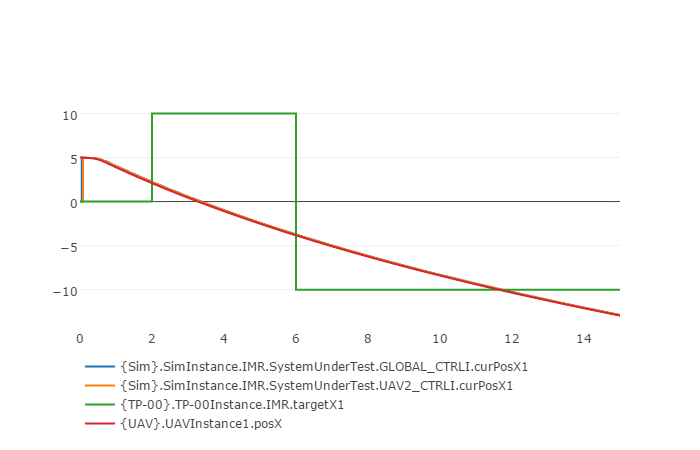
\includegraphics[width=1.0\textwidth]{uav_swarm_ta_ether_uav2_posX1}
%%    \caption{Target position and current position of UAV1 in the X axis}
%%    \label{fig:uav_swarm_ta_ether_uav2_posX1}
%%\end{figure}
%%
%%\begin{figure}[htb!]
%%    \centering
%%	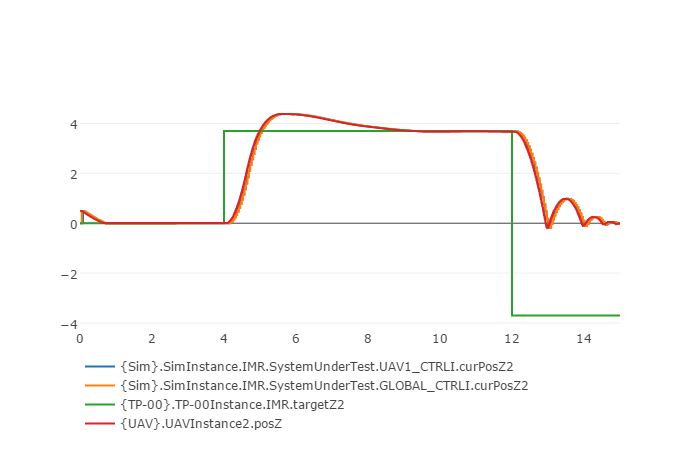
\includegraphics[width=1.0\textwidth]{uav_swarm_ta_ether_uav2_posZ2}
%%    \caption{Target position and current position of UAV2 in the Z axis}
%%    \label{fig:uav_swarm_ta_ether_uav2_posZ2}
%%\end{figure}

%\subparagraph{Approaching}
%Will the UAV approach its target position and how long?
%
%\paragraph{Co-simulation with 3-UAV-Non-3D}
%A co-simulation result is displayed in Figure~\ref{fig:uav_swarm_mm_3uav_100}.
%\begin{figure}[htb!]
%    \centering
%	\includegraphics[width=1.0\textwidth]{uav_swarm_multimodel_cosim_100}
%    \caption{Co-simulation result of 3-UAV-Non-3D}
%    \label{fig:uav_swarm_mm_3uav_100}
%\end{figure}
%
%\paragraph{Co-simulation: TP-00, SIM, and UAV (20-Sim)} This multi-model uses a UAV FMU from 20-sim as a part of test environment in a test run. In this configuration, 
%\begin{itemize}
%    \item $target$ positions from TP-00 are connected to SIM  
%    \item current $pos$ positions,  $vel$ velocities, and battery charge are connected from UAV to SIM  
%    \item outputs of SIM ($throttle$, $roll$, $yaw$, and $pitch$) are connected to UAV
%\end{itemize}
%
%A Co-simulation result is displayed in Figure~\ref{fig:uav_swarm_mm_tp00_sim_uav}.
%\begin{figure}[htb!]
%    \centering
%	\includegraphics[width=1.0\textwidth]{uav_swarm_multimodel_cosim_tp00_sim_uav_5}
%    \caption{Co-simulation result of TP00, SIM and UAV}
%    \label{fig:uav_swarm_mm_tp00_sim_uav}
%\end{figure}
%
%
%Some important points:
%\begin{itemize}
%    \item 
%    \item
%    \item
%\end{itemize}

%\subparagraph{A SUT with separate controller and multiple FMUs}
\subparagraph{Test Goals}
The test goal is defined by a user defined test case through the LTL formula: $Finally [\_timeTick \ge 25000]$. The \emph{Admissible Error} and \emph{Latency} in ``signalmap.csv'' are set to 0.0000001 and 5 ms respectively.

%\lstset{language={},
%    basicstyle=\scriptsize\ttfamily,
%    showstringspaces=false,
%    tabsize=2
%}
%\begin{lstlisting}
%{
%	"goals": [
%		{
%			"ltl-formula": "Finally ([_timeTick >= 25000])",
%			"ordered": false
%		}
%	],
%	"model-config": [
%
%	],
%	"solver-config": {
%		"abstract-interpretation": false,
%		"backtracking": false,
%		"cover-all-goals": true,
%		"ignore-test-oracles": false,
%		"max-simulation-steps": 0,
%		"max-solver-steps": 100,
%		"maximise-coverage": false,
%		"min-change-duration": 10,
%		"model-checking": false,
%		"robustness-percentage": 0,
%		"robustness-testing": false,
%		"sanity-checks": false,
%		"simultaneous-changes": 1,
%		"verbosity-level": 1
%	}
%}
%
%\end{lstlisting}
%
%``Admissible Error'' and ``Latency'' in ``signalmap.csv'' are set to 0.0000001 and 5ms.

\subparagraph{Co-Simulation without UAVs}
This test configuration is used to check if the SUT is a right implementation of the test model. The connection of five FMUs is configured as shown in Figure~\ref{fig:Connection_wo_UAVs}. This configuration does not include \emph{UAVs}. Instead, current positions and velocities from \emph{TP-00} are connected to corresponding ports in \emph{UAV Controllers}, and the UAV control signals ($throttle$, $roll$, $yaw$, and $pitch$) are connected from \emph{UAV Controllers} to \emph{TP-00}. Therefore, \emph{TP-00} has all outputs and inputs connected to the SUT. Finally, test results are able to check if behaviour between the SUT and the test model (in \emph{TP-00}) is consistent. Our test with used defined test case shows that all test cases are either \T{PASSED} or \T{INCONCLUSIVE}, and no \T{FAIL}. 

\begin{figure}[htb!]
    \centering
	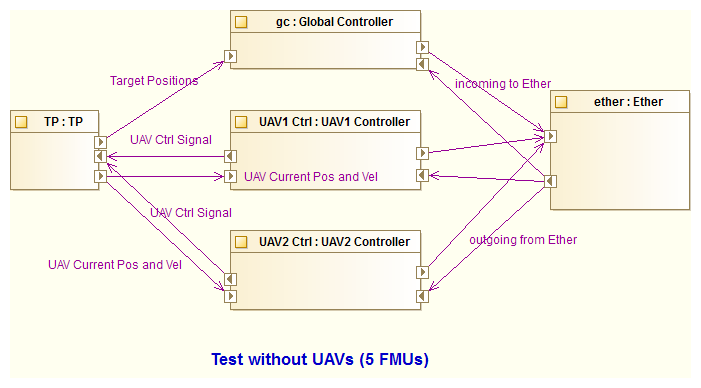
\includegraphics[width=1.0\textwidth]{test_conf/Connection_wo_UAVs}
    \caption{Connection for Test without UAVs}
    \label{fig:Connection_wo_UAVs}
\end{figure}

\subparagraph{Co-Simulation with UAVs}
This test configuration is not intended for checking SUT against the test model, but for Co-Simulation with physical \emph{UAVs} (20-sim models). The connection of seven FMUs is configured as shown in Figure~\ref{fig:Connection_UAVs}. There are two \emph{UAVs} and each of them is connected to corresponding \emph{UAV Controller}. 

Current positions and velocities to \emph{UAV Controllers} are from \emph{UAVs} and those from \emph{TP-00} are left unconnected. But we still connect UAVs control signals from \emph{UAV Controllers} to both \emph{TP-00} and \emph{UAVs}. This test is not able to check behaviour of the SUT against the test model because input sequences in expected results from \emph{TP-00} and actual results from SUT are different. %Obviously, the current positions and velocities generated are different from those from physical UAVs because the test model does not include physical hardware in loop. 
The test results show the RT Tester reports many \emph{FAILs}, almost all \textrm{FAILs} after initial match with zero.  

However, we can use this test configuration with Multi-model on the INTO-CPS application to co-simulate the UAV swarm in a context that all target positions are given from the test model by a state machine diagram of TestEnvironment.

\begin{figure}[htb!]
    \centering
	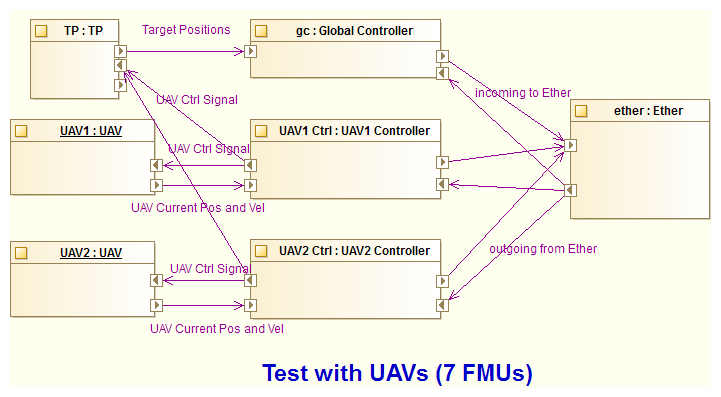
\includegraphics[width=1.0\textwidth]{test_conf/Connection_UAVs}
    \caption{Connection for Test with UAVs}
    \label{fig:Connection_UAVs}
\end{figure}

Co-Simulation results for \emph{UAV1} are displayed in Figure~\ref{fig:uav_swarm_7fmus_mm_UAV1}. This chart illustrates target positions in the X and Z axes (blue and orange respectively), current positions and velocities in the X and Z axes (green-yellow, grey, pink, and brown), and control signals from UAV controller ($throttle$ - green, $pitch$ - red, and $roll$ - purple). Several observations can be seen from this chart.
\begin{itemize}
    \item basically, current position ($posX1$ - green-yellow) of \emph{UAV1} follows its target position ($curPosX1$ - blue) though there is a delay,
    \item current position ($posZ1$ - grey) of \emph{UAV1} follows its target position ($curPosZ1$ - orange) when it is larger than 0, but current position won't go below 0. So \emph{UAVs} might have this restriction,
    \item velocities in the X and Z axes reflect movement of the \emph{UAVs} in the axes as well,
    \item and the changes of positions, directions and velocities are also driven by the changes in control signals ($throttle$, $picth$, and $roll$).
\end{itemize}

\begin{figure}[htb!]
    \centering
	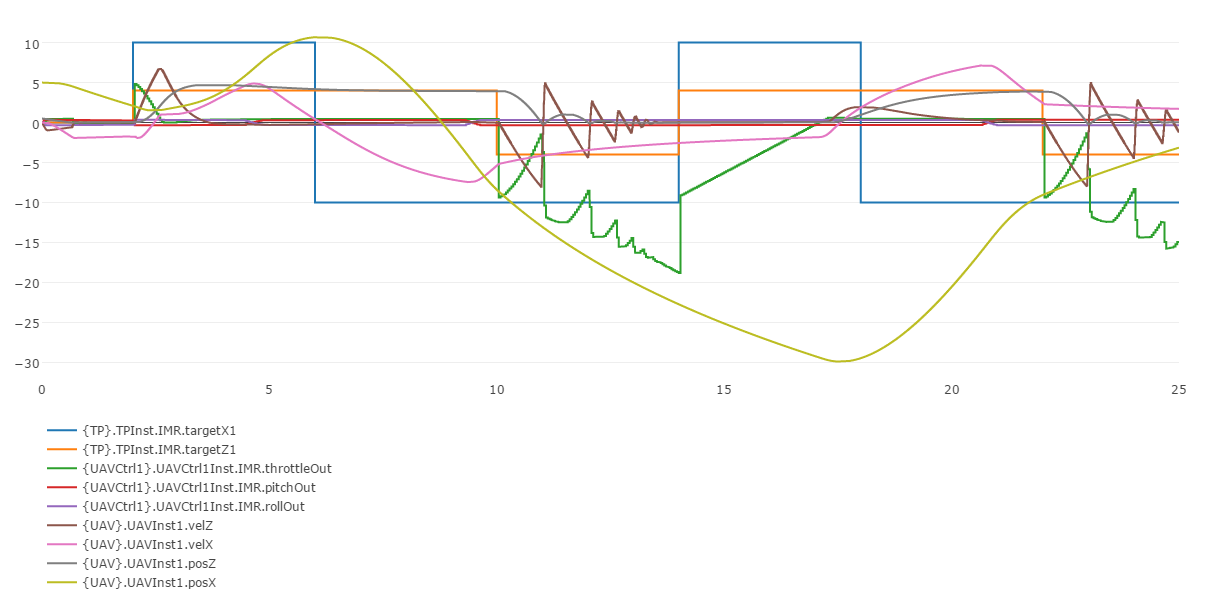
\includegraphics[width=1.0\textwidth]{SUTs_test_results/mm_X1_Z1_20170718}
    \caption{Co-Simulation Results of \emph{UAV1}}
    \label{fig:uav_swarm_7fmus_mm_UAV1}
\end{figure}

Co-Simulation results for \emph{UAV2} is displayed in Figure~\ref{fig:uav_swarm_7fmus_mm_UAV2}. This chart illustrates similar observations as Figure~\ref{fig:uav_swarm_7fmus_mm_UAV1}.

\begin{figure}[htb!]
    \centering
	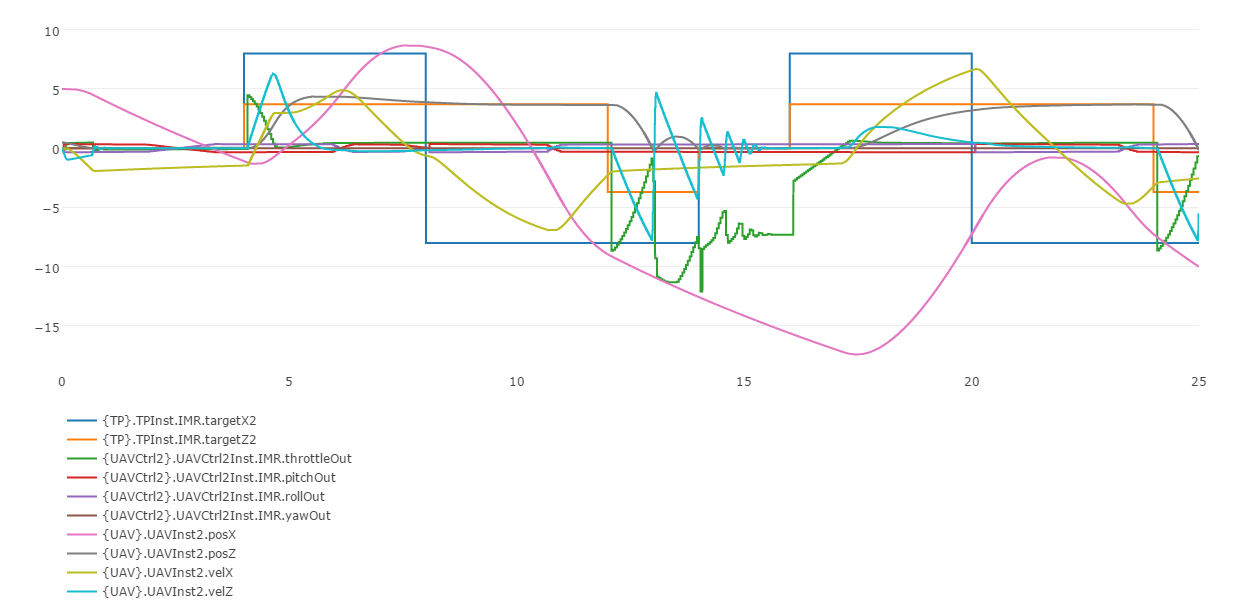
\includegraphics[width=1.0\textwidth]{SUTs_test_results/mm_X2_Z2_20170718}
    \caption{Co-Simulation Results of \emph{UAV2}}
    \label{fig:uav_swarm_7fmus_mm_UAV2}
\end{figure}



